\chapter{最小生成樹}
\label{ch:mst}

% 本章的圖共用的樣式（前綴 mst-）。 追蹤表、圖上的粗線和程式輸出都由模擬程式照虛擬碼
% 逐步執行後產生，再和本章的 C 程式輸出對過。
\tikzset{
    mst-v/.style={circle, draw=black!70, fill=white, minimum size=0.62cm, inner sep=0pt, font=\small},
    mst-e/.style={draw=black!50, thick},
    mst-t/.style={draw=black, line width=1.6pt},
    mst-x/.style={draw=black!35, densely dashed},
    mst-w/.style={font=\scriptsize, fill=white, inner sep=1pt},
    mst-cross/.style={draw=memStroke, line width=1.4pt},
    mst-light/.style={draw=optStroke, line width=2.2pt},
    mst-new/.style={draw=optStroke, line width=1.6pt},
    mst-side/.style={rounded corners=8pt, fill=coreFill, draw=coreStroke!50},
    mst-hull/.style={line width=0.95cm, line cap=round, line join=round, draw=coreFill, fill=coreFill},
    mst-lab/.style={font=\scriptsize, text=black!80},
    mst-pick/.style={-{Stealth[length=2mm]}, draw=optStroke, thick, shorten >=1pt},
}
% Prim 追蹤表：框起來的是這一回合取出的頂點，底色是這一回合改過的 key。
\newcommand{\mstsel}[1]{\fbox{#1}}
\newcommand{\mstchg}[1]{\colorbox{memFill}{#1}}

山上的露營區有八個營地，管理處打算拉電線，讓每個營地都有電。 電只要能從一個營地經過
別的營地送過來就好，不需要每兩個營地之間都有線。 工程行估了價：有些營地之間地形平
緩，拉線便宜；有些要跨過溪谷，貴很多；還有些營地之間根本拉不過去。 管理處想用最少
的錢，讓八個營地全部連在一起。 往下讀之前，先想想：從最便宜的那段開始拉，一段一段
加上去，最後的總價會是最少的嗎？ 如果不是每段都要，哪些段可以放心跳過？

這一章處理的就是這個問題：在一張每條邊都有權重的連通無向圖裡，挑出一些邊把所有頂點
連起來，而且總權重最小。 挑出來的一定是一棵生成樹，叫做\textbf{最小生成樹}。 我們
先證明兩個性質：\textbf{切割性質}告訴我們哪些邊一定可以放心選，\textbf{環性質}告訴我們
哪些邊可以放心不選。 三個經典演算法都是切割性質的應用，差別只在每次看哪一個切割：
Kruskal 演算法把邊由輕到重排好，一條一條試；Prim 演算法從一個頂點開始，把樹往外長；
Sollin 演算法（也叫 Borůvka 演算法）讓每個元件同時挑一條最輕的邊。 最後談幾個考試常
問的觀念：權重相同時怎麼處理、最小生成樹什麼時候唯一、次小生成樹，以及最小生成樹和最
短路徑樹為什麼不一樣。

這一章用到前面的這些東西：第~21~章的生成樹、樹的等價性質（定理~\ref{thm:gtr-tree}：$n$ 個頂點的樹恰好有
$n - 1$ 條邊、任兩點之間恰好一條簡單路徑）和鄰接串列；第~13~章的互斥集合；第~8~章的帶索
引最小堆積和 \proc{Decrease-Key}；第~19~章的貪心法和交換論證。 程式方面用到《C 程式
設計基礎》第~14~章的結構、第~19~章的 \texttt{malloc} 和鏈結串列，以及標準函式庫的
\texttt{qsort}。

本章的約定和第~21~章相同：圖是\textbf{連通的簡單無向圖}，有 $n$ 個頂點、$m$ 條邊，頂點
編號 $1$ 到 $n$（觀念題有時用英文字母）；每條邊 $(u, v)$ 有一個權重 $w(u, v)$，可以是
任何實數，包括 $0$ 和負數。 鄰接串列裡的鄰居由小到大排。 C 程式裡的頂點從 $0$ 編號，讀
入時減一、印出時加一。

\section{最小生成樹與兩個性質}
\label{sec:mst-props}

\subsection{問題}

對一個邊的集合 $A$，令 $w(A) = \sum_{(u, v) \in A} w(u, v)$，叫做 $A$ 的\textbf{總權
重}。

\begin{definition}
$G = (V, E)$ 是連通的無向圖，每條邊有權重 $w$。 $G$ 的生成樹 $T$ 裡，總權重 $w(T)$ 最
小的叫做 $G$ 的\textbf{最小生成樹}（minimum spanning tree，簡稱 MST）。 $G$ 不連通時，
每個連通元件各取一棵最小生成樹，合起來叫\textbf{最小生成森林}。
\end{definition}

由第~21~章樹的等價性質（定理~\ref{thm:gtr-tree}），每一棵生成樹都恰好有 $n - 1$ 條邊，所以「總權重最小」比的是同
樣多條邊的總和。 最小生成樹不一定只有一棵：權重相同的邊可能互相替換，總權重一樣。 「最
小」指的是總權重，不是邊數，也不是最重的那條邊。

\begin{center}
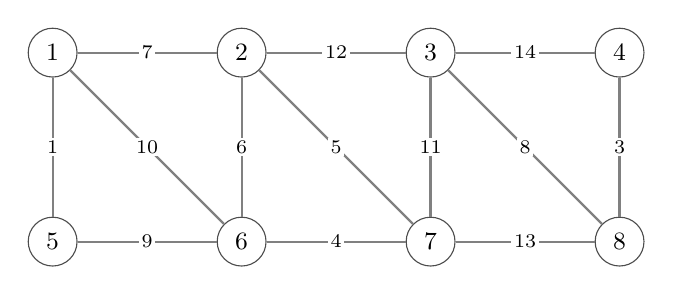
\begin{tikzpicture}[x=1.2cm, y=1.2cm]
\node[mst-v] (v1) at (0,2) {$1$};
\node[mst-v] (v2) at (2,2) {$2$};
\node[mst-v] (v3) at (4,2) {$3$};
\node[mst-v] (v4) at (6,2) {$4$};
\node[mst-v] (v5) at (0,0) {$5$};
\node[mst-v] (v6) at (2,0) {$6$};
\node[mst-v] (v7) at (4,0) {$7$};
\node[mst-v] (v8) at (6,0) {$8$};
\draw[mst-e] (v1) -- node[mst-w] {7} (v2);
\draw[mst-e] (v2) -- node[mst-w] {12} (v3);
\draw[mst-e] (v3) -- node[mst-w] {14} (v4);
\draw[mst-e] (v5) -- node[mst-w] {9} (v6);
\draw[mst-e] (v6) -- node[mst-w] {4} (v7);
\draw[mst-e] (v7) -- node[mst-w] {13} (v8);
\draw[mst-e] (v1) -- node[mst-w] {1} (v5);
\draw[mst-e] (v2) -- node[mst-w] {6} (v6);
\draw[mst-e] (v3) -- node[mst-w] {11} (v7);
\draw[mst-e] (v4) -- node[mst-w] {3} (v8);
\draw[mst-e] (v1) -- node[mst-w] {10} (v6);
\draw[mst-e] (v2) -- node[mst-w] {5} (v7);
\draw[mst-e] (v3) -- node[mst-w] {8} (v8);
\end{tikzpicture}
\diagcaption{露營區的八個營地。 每條邊是一段拉得過去的電線，數字是費用（萬元）。 本章的
Kruskal、Prim、Sollin 三個演算法都在這張圖上追蹤。}
\label{fig:mst-camp}
\end{center}

圖~\ref{fig:mst-camp} 是章首的露營區，記成 $G$。 它有 $13$ 條邊，每棵生成樹要挑其中 $7$
條；用程式列舉，一共有 $377$ 棵生成樹。 一棵一棵算總權重太慢，需要一套挑邊的規則，而且
要能證明它不會挑錯。

最直接的想法是貪心：從最便宜的邊開始拉，會形成環的就跳過。 $1$--$5$（$1$）、$4$--$8$
（$3$）、$6$--$7$（$4$）、$2$--$7$（$5$）都可以拉；接下來 $2$--$6$（$6$）的兩端已經經過
$7$ 連在一起，拉了只會多花錢……這就是第~\ref{sec:mst-kruskal}~節的 Kruskal 演算法。 它
看起來合理，但第~19~章說過，貪心法每一步都要證明不會錯。 證明的工具是下面的切割性質。

\subsection{切割}

\begin{definition}
把頂點分成兩個都不是空的集合 $S$ 和 $V - S$，叫做一個\textbf{切割}（cut），寫成 $(S, V -
S)$。 一條邊的兩端一個在 $S$、一個在 $V - S$，就說這條邊\textbf{跨越}這個切割。 跨越
切割的邊裡，權重最小的叫做這個切割的\textbf{輕邊}（light edge）；權重最小的邊有好幾條
時，每一條都是輕邊。 如果邊集合 $A$ 裡沒有任何一條邊跨越切割，就說這個切割\textbf{尊
重} $A$。
\end{definition}

\begin{center}
\begin{tikzpicture}[x=1.2cm, y=1.2cm]
\node[mst-v] (v1) at (0,2) {$1$};
\node[mst-v] (v2) at (2,2) {$2$};
\node[mst-v] (v3) at (4,2) {$3$};
\node[mst-v] (v4) at (6,2) {$4$};
\node[mst-v] (v5) at (0,0) {$5$};
\node[mst-v] (v6) at (2,0) {$6$};
\node[mst-v] (v7) at (4,0) {$7$};
\node[mst-v] (v8) at (6,0) {$8$};
\begin{scope}[on background layer]
\node[mst-side, fit=(v1)(v2)(v5)(v6), inner sep=7pt] (S) {};
\end{scope}
\draw[mst-e] (v1) -- node[mst-w] {7} (v2);
\draw[mst-cross] (v2) -- node[mst-w] {12} (v3);
\draw[mst-e] (v3) -- node[mst-w] {14} (v4);
\draw[mst-e] (v5) -- node[mst-w] {9} (v6);
\draw[mst-light] (v6) -- node[mst-w] {4} (v7);
\draw[mst-e] (v7) -- node[mst-w] {13} (v8);
\draw[mst-e] (v1) -- node[mst-w] {1} (v5);
\draw[mst-e] (v2) -- node[mst-w] {6} (v6);
\draw[mst-e] (v3) -- node[mst-w] {11} (v7);
\draw[mst-e] (v4) -- node[mst-w] {3} (v8);
\draw[mst-e] (v1) -- node[mst-w] {10} (v6);
\draw[mst-cross] (v2) -- node[mst-w] {5} (v7);
\draw[mst-e] (v3) -- node[mst-w] {8} (v8);
\node[mst-lab, anchor=south] at (S.north) {$S$};
\node[mst-lab, anchor=south] at ($(v3)!0.5!(v4)+(0,0.45)$) {$V - S$};
\end{tikzpicture}
\diagcaption{切割 $(S, V - S)$，$S = \{1, 2, 5, 6\}$。 跨越它的邊有三條（橘色）：
$6$--$7$（$4$）、$2$--$7$（$5$）、$2$--$3$（$12$）。 輕邊是 $6$--$7$（紅色）。}
\label{fig:mst-cut}
\end{center}

圖~\ref{fig:mst-cut} 是一個例子。 不管最後的生成樹長什麼樣子，它一定要用到至少一條跨越
這個切割的邊，否則 $S$ 和 $V - S$ 就不相連了。 直覺上，既然一定要過去，就挑最便宜的那條
過去。 下面的定理說這個直覺是對的，而且可以在「已經選了一些邊」的情況下繼續用。

\subsection{切割性質}

在證明之前先定一個說法。 $A$ 是一些邊的集合，而且 $A$ 包含在某一棵最小生成樹裡。 如果
再加一條邊 $(u, v)$，$A \cup \{(u, v)\}$ 仍然包含在某一棵最小生成樹裡，就說 $(u, v)$
對 $A$ 是\textbf{安全的}（safe）。 從 $A = \emptyset$ 開始，每次加一條安全的邊，加了 $n
- 1$ 條之後，$A$ 本身就是一棵最小生成樹。

\begin{theorem}[切割性質]
\label{thm:mst-cut}
$G$ 是連通的加權無向圖，邊集合 $A$ 包含在 $G$ 的某一棵最小生成樹裡。 $(S, V - S)$ 是尊
重 $A$ 的任何一個切割，$(u, v)$ 是這個切割的一條輕邊。 那麼 $(u, v)$ 對 $A$ 是安全的。
\end{theorem}

\begin{proof}
令 $T$ 是包含 $A$ 的一棵最小生成樹。 如果 $(u, v) \in T$，$T$ 本身就包含 $A \cup \{(u,
v)\}$，得證。

否則把 $(u, v)$ 加進 $T$。 $T$ 裡 $u$ 到 $v$ 本來就有一條簡單路徑 $P$，加上 $(u, v)$ 就
形成一個環。 $u$ 和 $v$ 一個在 $S$、一個在 $V - S$，所以 $P$ 從 $S$ 出發、走到 $V - S$，
途中至少有一條邊 $(x, y)$ 跨越這個切割。 這條邊有三個性質：
\begin{itemize}
\item $(x, y) \notin A$，因為切割尊重 $A$，$A$ 裡沒有跨越切割的邊；
\item $w(u, v) \le w(x, y)$，因為 $(u, v)$ 是輕邊，而 $(x, y)$ 也跨越切割；
\item $(x, y) \ne (u, v)$，因為 $(x, y)$ 在 $T$ 裡，$(u, v)$ 不在。
\end{itemize}
令 $T' = T - \{(x, y)\} \cup \{(u, v)\}$。 從 $T$ 拿掉 $(x, y)$，樹分成兩塊，一塊含 $x$、
一塊含 $y$；$u$、$v$ 分別在這兩塊（路徑 $P$ 被切斷的兩邊），加上 $(u, v)$ 又連成一棵
樹，所以 $T'$ 是生成樹。 它的總權重
\[
w(T') = w(T) - w(x, y) + w(u, v) \le w(T),
\]
而 $T$ 已經是最小的，所以 $w(T') = w(T)$，$T'$ 也是最小生成樹。 $A \subseteq T$ 而且
$(x, y) \notin A$，所以 $A \subseteq T'$，再加上 $(u, v) \in T'$，得證。
\end{proof}

證明裡的動作「加一條邊形成環，再從環上拿掉另一條」叫做\textbf{換邊}，本章會一直用到。
它是第~19~章交換論證在生成樹上的版本：換完之後要說明兩件事，結果仍然是生成樹，而且總權
重沒有變大。

取 $A = \emptyset$，任何切割都尊重它，得到一個常用的特例。

\begin{corollary}
\label{cor:mst-cut-strict}
任何一個切割的輕邊，都屬於某一棵最小生成樹。 如果一個切割的輕邊只有一條（權重嚴格最
小），它屬於\textbf{每一棵}最小生成樹。
\end{corollary}

\begin{proof}
第一句是定理~\ref{thm:mst-cut} 取 $A = \emptyset$。 第二句：假設某棵最小生成樹 $T$ 不含
這條唯一的輕邊 $(u, v)$，照上面的證明換邊，換掉的 $(x, y)$ 跨越切割、又不是 $(u, v)$，
所以 $w(x, y) > w(u, v)$，$w(T') < w(T)$，和 $T$ 最小矛盾。
\end{proof}

在圖~\ref{fig:mst-cut} 裡，$6$--$7$ 是唯一的輕邊，所以每一棵最小生成樹都有 $6$--$7$。 把
$S$ 換成 $\{v\}$（一個頂點自己一邊），就得到：\textbf{每個頂點連出去的邊裡最輕的那一條，
一定在某一棵最小生成樹裡}。 第~\ref{sec:mst-sollin}~節的 Sollin 演算法第一回合就是靠這
件事。

\subsection{環性質}

切割性質說哪些邊可以選，環性質說哪些邊可以不選。

\begin{theorem}[環性質]
\label{thm:mst-cycle}
$C$ 是 $G$ 裡的一個環，$e$ 是 $C$ 上權重最大的一條邊（$C$ 上其他邊的權重都 $\le w(e)$）。
那麼 $G$ 有一棵最小生成樹不含 $e$。 如果 $e$ 是 $C$ 上\textbf{唯一}權重最大的邊，$e$ 不在
任何一棵最小生成樹裡。
\end{theorem}

\begin{proof}
令 $T$ 是一棵最小生成樹，$e = (u, v)$。 如果 $e \notin T$，第一句已經成立。 設 $e \in
T$。 從 $T$ 拿掉 $e$，樹分成兩塊，令 $S$ 是含 $u$ 的那一塊的頂點，$v \in V - S$。 環 $C$
拿掉 $e$ 之後是一條從 $u$ 到 $v$ 的路徑，這條路徑從 $S$ 走到 $V - S$，一定有一條邊 $f$ 跨越
$(S, V - S)$，而且 $f \ne e$。 $T$ 裡跨越這個切割的邊只有 $e$（$T - \{e\}$ 的兩塊之間沒
有別的邊），所以 $f \notin T$。

$T' = T - \{e\} \cup \{f\}$ 又把兩塊連起來，是一棵生成樹，$w(T') = w(T) - w(e) + w(f)$。
$f$ 也在環 $C$ 上，$w(f) \le w(e)$，所以 $w(T') \le w(T)$，$T'$ 是不含 $e$ 的最小生成樹。
如果 $e$ 是唯一最大的，$w(f) < w(e)$，$w(T') < w(T)$，和 $T$ 最小矛盾，所以 $T$ 根本不能
含 $e$。
\end{proof}

在圖~\ref{fig:mst-camp} 裡，環 $2 \to 6 \to 7 \to 2$ 的三條邊是 $6$、$4$、$5$，$2$--$6$
（$6$）唯一最重，所以 $2$--$6$ 不在任何最小生成樹裡。 環性質也可以反過來用：依權重由大
到小看每條邊，拿掉之後圖還連通（也就是它在某個環上，而且是那個環上最重的）就拿掉。 這
個做法叫\textbf{反向刪除}（reverse-delete），結果一樣是最小生成樹，但每次都要檢查連通，
比本章的三個演算法慢。 有些中文教材叫它「破圈法」。

\subsection{通用的做法}

三個演算法都套用同一個骨架：維護一個邊的集合 $A$，保持「$A$ 包含在某一棵最小生成樹
裡」，每次加一條安全的邊。

\begin{pseudo}[label=alg:mst-generic]{通用的最小生成樹做法}
\Procedure{Generic-MST}{$G, w$}
    \State $A \gets \emptyset$
    \While{$A$ 還不是一棵生成樹}
        \State 找一條對 $A$ 安全的邊 $(u, v)$
        \State $A \gets A \cup \{(u, v)\}$
    \EndWhile
    \State \Return $A$
\EndProcedure
\end{pseudo}

$A$ 在過程中一直是一個森林（沒有環），它的每個連通元件是一棵樹。 第 4 行怎麼找，就是
三個演算法的差別：

\begin{center}
\small
\begin{tabular}{lll}
\toprule
演算法 & $A$ 的樣子 & 用哪個切割 \\
\midrule
Kruskal & 好幾棵樹組成的森林 & 下一條要加的邊的一端所在的那棵樹 vs. 其他 \\
Prim & 從起點長出來的一棵樹 & 這棵樹 vs. 其他頂點 \\
Sollin & 好幾棵樹組成的森林 & 每棵樹各自 vs. 其他，同時進行 \\
\bottomrule
\end{tabular}
\end{center}

第~\ref{sec:gr-matroid}~節介紹過擬陣。 圖的邊、以「不含環」為獨立的條件，構成一個擬陣（圖擬陣），所以依權
重由小到大的貪心一定對，這是 Kruskal 演算法正確的另一種說法。 本章用切割性質證明，因為
它同時涵蓋三個演算法。

\subsection{權重互不相同時，最小生成樹唯一}

\begin{theorem}
\label{thm:mst-unique}
如果 $G$ 每條邊的權重都不相同，$G$ 的最小生成樹只有一棵。
\end{theorem}

\begin{proof}
假設 $T_1 \ne T_2$ 都是最小生成樹。 兩者都有 $n - 1$ 條邊，所以兩邊各有對方沒有的邊。 在
所有「恰好屬於其中一棵」的邊裡，取權重最小的一條 $e$；權重互不相同，$e$ 是唯一的。 不
妨設 $e \in T_1$、$e \notin T_2$。

把 $e$ 加進 $T_2$ 形成一個環。 這個環上一定有一條邊 $f$ 不在 $T_1$ 裡，否則整個環都在
$T_1$ 裡，和 $T_1$ 是樹矛盾。 $f$ 在 $T_2$ 裡而不在 $T_1$ 裡，也是「恰好屬於其中一棵」的
邊，又 $f \ne e$，由 $e$ 的取法，$w(f) > w(e)$。 和切割性質的證明一樣，$T_2 - \{f\} \cup
\{e\}$ 是一棵生成樹，總權重 $w(T_2) - w(f) + w(e) < w(T_2)$，和 $T_2$ 最小矛盾。
\end{proof}

反過來不成立：權重有相同的，最小生成樹仍然可能唯一。 例如三角形的三條邊權重是 $1$、$1$、
$2$，最小生成樹只有 $\{1, 1\}$ 那一棵（權重 $2$ 的邊是環上唯一最重的，由環性質一定不選）。
更極端的例子是 $G$ 本身就是一棵樹，不管權重是多少，最小生成樹都是它自己。
第~\ref{sec:mst-more}~節會給一個「最小生成樹唯一」的充分必要條件。

另外，最小生成樹不唯一時，每一棵的總權重當然相同。 更強的事也成立（這裡不證）：把每一
棵的邊權重由小到大排成一列，得到的數列都一樣。 例如某張圖的一棵最小生成樹用了兩段 $3$ 萬、
一段 $5$ 萬，另一棵最小生成樹也一定是兩段 $3$ 萬、一段 $5$ 萬，只是選的位置不同。

\subsection{權重相同時：平手規則}
\label{sec:mst-ties}

考試和程式裡的圖常常有權重相同的邊。 這時最小生成樹可能不只一棵，演算法選哪一棵取決於
平手時怎麼排。 本書的約定是：每條邊寫成 $(u, v)$ 且 $u < v$，兩條邊比較時

\begin{enumerate}
\item 權重小的比較「輕」；
\item 權重相同時，$u$（小的端點）小的比較輕；
\item 權重和 $u$ 都相同時，$v$（大的端點）小的比較輕。
\end{enumerate}

用字母當頂點時，照字母順序。 這樣任兩條不同的邊都分得出輕重，寫成 $e \prec f$（$e$ 比 $f$
輕）。 Kruskal 演算法排序和 Sollin 演算法挑邊都照 $\prec$。 Prim 演算法比的是頂點的
$\mathit{key}$，它的平手規則另外在第~\ref{sec:mst-prim}~節說明。

\begin{lemma}
\label{lem:mst-ties}
照 $\prec$ 比輕重，就好像所有權重都不相同：在 $\prec$ 之下最輕的生成樹 $T_{\prec}$ 只
有一棵，而且 $T_{\prec}$ 是 $G$（原本的權重）的一棵最小生成樹。
\end{lemma}

\begin{whybox}[引理~\ref{lem:mst-ties}]
把邊照 $\prec$ 由輕到重排成 $e_1, e_2, \ldots, e_m$，令 $r(e_i) = i$。 取一個很小的正
數 $\varepsilon$，定義新的權重
\[
w'(e) = w(e) + \varepsilon \cdot r(e).
\]
先看權重都是整數的情況（考試的圖幾乎都是），取 $\varepsilon = 1/(mn)$。
\begin{itemize}
\item \textbf{$w'$ 互不相同，而且大小順序就是 $\prec$}：$w(e) < w(f)$ 時 $w(f) - w(e) \ge
1$，而 $\varepsilon\,|r(e) - r(f)| < \varepsilon m < 1$，所以 $w'(e) < w'(f)$；$w(e) = w(f)$
時由 $r$ 決定。 所以照 $\prec$ 比較，等於照 $w'$ 比較。
\item \textbf{$w'$ 的最小生成樹也是 $w$ 的最小生成樹}：任何一棵生成樹 $T$ 有 $n - 1$ 條
邊，$0 < w'(T) - w(T) = \varepsilon \sum_{e \in T} r(e) \le \varepsilon \cdot (n - 1) m < 1$。
設 $T'$ 是 $w'$ 的最小生成樹，$T$ 是任何一棵生成樹。 如果 $w(T) < w(T')$，因為都是整數，
$w(T) \le w(T') - 1$，於是 $w'(T) < w(T) + 1 \le w(T') < w'(T')$，和 $T'$ 對 $w'$ 最小矛
盾。 所以 $w(T') \le w(T)$。
\end{itemize}
$w'$ 的權重互不相同，由定理~\ref{thm:mst-unique}，它的最小生成樹只有一棵，就是 $T_{\prec}$。

權重是一般實數時，把上面的「$1$」換成「兩條邊權重的差」和「兩棵生成樹總權重的差」裡最
小的正數（有限多個，一定有最小值），$\varepsilon$ 取得比這個數除以 $mn$ 還小，論證完全
相同。
\end{whybox}

所以只要所有比較都照 $\prec$ 做，演算法就像在一張權重互不相同的圖上執行，結果一定是
$T_{\prec}$ 這一棵。 第~\ref{sec:mst-kruskal}~節的 Kruskal 演算法和第~\ref{sec:mst-sollin}~節
的 Sollin 演算法都是這樣，對同一張圖會選出同一棵樹。

\begin{examnote}
權重相同時，「最小生成樹是哪一棵」的答案不只一個，所以追蹤題通常會規定平手時怎麼排（例
如「權重相同時先選頂點編號小的邊」「權重相同時依字母順序」「Prim 演算法權重相同時先加入
編號小的頂點」）。 不同課本的約定不同，照題目寫；題目沒規定時，在答案開頭寫明自己用的規
則，例如本書的「先比權重，再比小端點，再比大端點」。 問總權重時答案只有一個，不受平手規
則影響。
\end{examnote}

\section{Kruskal 演算法}
\label{sec:mst-kruskal}

Kruskal 演算法就是第~\ref{sec:mst-props}~節開頭那個貪心：把邊依權重由小到大排好，一條一
條看；兩端已經連通的邊會形成環，跳過，否則選進來。 「兩端是不是已經連通」用第~13~章的互
斥集合判斷：每個集合是目前森林裡一棵樹的頂點，\proc{Find-Set} 找代表，\proc{Union} 把兩
棵樹併起來。

\begin{pseudo}[label=alg:mst-kruskal]{Kruskal 演算法}
\Procedure{MST-Kruskal}{$G, w$}
    \State $A \gets \emptyset$
    \For{每個頂點 $v \in G.V$}
        \State \Call{Make-Set}{$v$}
    \EndFor
    \State 把 $G.E$ 的邊照 $\prec$ 由輕到重排序 \Comment{第~\ref{sec:mst-ties}~節的平手規則}
    \For{依排好的順序，每條邊 $(u, v)$}
        \If{$\Call{Find-Set}{u} \ne \Call{Find-Set}{v}$}
            \State $A \gets A \cup \{(u, v)\}$
            \State \Call{Union}{$u, v$}
        \EndIf
    \EndFor
    \State \Return $A$
\EndProcedure
\end{pseudo}

第 7 行的判斷就是第~21~章引理~\ref{lem:gtr-count}（邊數和連通元件數）的兩種情形：兩端已經在同一個集合，
加進來會形成環；兩端在不同集合，加進來會把兩棵樹接成一棵，集合數減一。 選滿 $n - 1$ 條
邊時已經是一棵生成樹，後面的邊一定都會跳過，可以提早結束迴圈。

\begin{theorem}
\label{thm:mst-kruskal}
$G$ 連通時，\proc{MST-Kruskal} 回傳一棵最小生成樹。 而且只要排序時平手照 $\prec$，回傳
的就是引理~\ref{lem:mst-ties} 的 $T_{\prec}$。
\end{theorem}

\begin{proof}
證明第 8 行每次加進來的邊對 $A$ 都是安全的。 設第 8 行要加 $(u, v)$，這時 $u$ 和 $v$ 在 $A$
的不同的樹裡。 令 $S$ 是 $u$ 所在那棵樹的頂點，$v \in V - S$。

\begin{itemize}
\item 切割 $(S, V - S)$ 尊重 $A$：$S$ 是 $A$ 的一個連通元件，$A$ 的邊不會一端在裡面、一
端在外面。
\item $(u, v)$ 跨越這個切割，而且是輕邊。 比 $(u, v)$ 早處理的每條邊，處理時要嘛被加進
$A$，要嘛兩端已經在同一棵樹裡；森林只會越併越大，所以現在它的兩端仍在同一棵樹裡，也就是
不跨越 $(S, V - S)$。 因此跨越切割的邊都排在 $(u, v)$ 或它後面，權重都 $\ge w(u, v)$。
\end{itemize}

由定理~\ref{thm:mst-cut}，$(u, v)$ 是安全的。 一開始 $A = \emptyset$ 包含在任何一棵最小生成
樹裡，歸納下去，$A$ 始終包含在某一棵最小生成樹裡。 最後 $A$ 是一棵生成樹：如果 $A$ 還有兩
棵以上的樹，$G$ 連通，一定有一條邊連接兩棵不同的樹，它被處理時兩端在不同集合，會被選進
來，矛盾。 一棵生成樹包含在某一棵最小生成樹裡，邊數又一樣，兩者相等。

照 $\prec$ 排序時，演算法的每個判斷都和「在 $w'$ 上執行」相同，而 $w'$ 的最小生成樹只有
$T_{\prec}$ 一棵（引理~\ref{lem:mst-ties}），所以回傳的是 $T_{\prec}$。
\end{proof}

圖不連通時，演算法照樣跑完，得到的是最小生成森林：證明裡的每一步都沒有用到連通，只有
最後「只剩一棵樹」那一步要用。 選到的邊數是 $n$ 減去連通元件數。

\subsection{手算追蹤}

在圖~\ref{fig:mst-camp} 的露營區上跑一次。 $13$ 條邊的權重都不同，排序不用平手規則。
下表一列是一條邊；最後一欄是處理完這條邊之後，互斥集合裡有兩個頂點以上的集合（其他頂點
各自一組）。

\begin{center}
\small
\begin{tabular}{rcrll}
\toprule
步 & 邊 & 權重 & 結果 & 處理完的集合 \\
\midrule
1 & $1$--$5$ & 1 & 選 & $\{1, 5\}$ \\
2 & $4$--$8$ & 3 & 選 & $\{1, 5\}$、$\{4, 8\}$ \\
3 & $6$--$7$ & 4 & 選 & $\{1, 5\}$、$\{4, 8\}$、$\{6, 7\}$ \\
4 & $2$--$7$ & 5 & 選 & $\{1, 5\}$、$\{2, 6, 7\}$、$\{4, 8\}$ \\
5 & $2$--$6$ & 6 & 略過（成環） & $\{1, 5\}$、$\{2, 6, 7\}$、$\{4, 8\}$ \\
6 & $1$--$2$ & 7 & 選 & $\{1, 2, 5, 6, 7\}$、$\{4, 8\}$ \\
7 & $3$--$8$ & 8 & 選 & $\{1, 2, 5, 6, 7\}$、$\{3, 4, 8\}$ \\
8 & $5$--$6$ & 9 & 略過（成環） & $\{1, 2, 5, 6, 7\}$、$\{3, 4, 8\}$ \\
9 & $1$--$6$ & 10 & 略過（成環） & $\{1, 2, 5, 6, 7\}$、$\{3, 4, 8\}$ \\
10 & $3$--$7$ & 11 & 選 & $\{1, 2, 3, 4, 5, 6, 7, 8\}$ \\
11--13 & \multicolumn{4}{l}{$2$--$3$（$12$）、$7$--$8$（$13$）、$3$--$4$（$14$）：已經選滿 $7$ 條，不用再看} \\
\bottomrule
\end{tabular}
\end{center}

\begin{center}
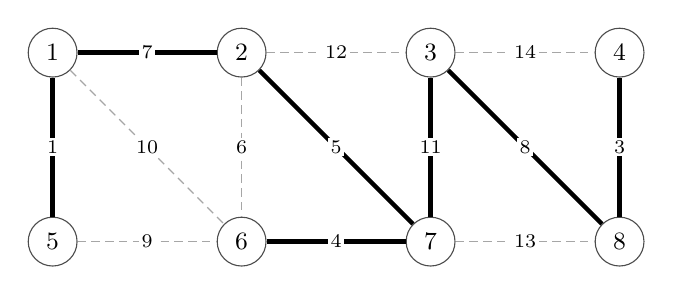
\begin{tikzpicture}[x=1.2cm, y=1.2cm]
\node[mst-v] (v1) at (0,2) {$1$};
\node[mst-v] (v2) at (2,2) {$2$};
\node[mst-v] (v3) at (4,2) {$3$};
\node[mst-v] (v4) at (6,2) {$4$};
\node[mst-v] (v5) at (0,0) {$5$};
\node[mst-v] (v6) at (2,0) {$6$};
\node[mst-v] (v7) at (4,0) {$7$};
\node[mst-v] (v8) at (6,0) {$8$};
\draw[mst-t] (v1) -- node[mst-w] {7} (v2);
\draw[mst-x] (v2) -- node[mst-w] {12} (v3);
\draw[mst-x] (v3) -- node[mst-w] {14} (v4);
\draw[mst-x] (v5) -- node[mst-w] {9} (v6);
\draw[mst-t] (v6) -- node[mst-w] {4} (v7);
\draw[mst-x] (v7) -- node[mst-w] {13} (v8);
\draw[mst-t] (v1) -- node[mst-w] {1} (v5);
\draw[mst-x] (v2) -- node[mst-w] {6} (v6);
\draw[mst-t] (v3) -- node[mst-w] {11} (v7);
\draw[mst-t] (v4) -- node[mst-w] {3} (v8);
\draw[mst-x] (v1) -- node[mst-w] {10} (v6);
\draw[mst-t] (v2) -- node[mst-w] {5} (v7);
\draw[mst-t] (v3) -- node[mst-w] {8} (v8);
\end{tikzpicture}
\diagcaption{露營區的最小生成樹（粗線），總權重 $1 + 3 + 4 + 5 + 7 + 8 + 11 = 39$。 虛線是沒有
選的邊。}
\label{fig:mst-tree}
\end{center}

幾個要注意的地方：

\begin{itemize}
\item 第 5 步的 $2$--$6$ 雖然只有 $6$ 萬，但 $2$、$6$ 已經經過 $7$ 連通了，拉了只是多一
條備用線。 這正是環性質：環 $2, 6, 7$ 上它最重。
\item 第 10 步的 $3$--$7$ 要 $11$ 萬，比被跳過的 $5$--$6$、$1$--$6$ 都貴，卻一定要選：它是
切割 $(\{1, 2, 5, 6, 7\}, \{3, 4, 8\})$ 的輕邊，跨越這個切割的另外兩條 $2$--$3$、$7$--$8$
更貴。 最小生成樹不是「挑最便宜的 $n - 1$ 條邊」。
\item 結果和第~\ref{sec:mst-props}~節開頭的貪心一模一樣，總共 $39$ 萬。 權重互不相同，由
定理~\ref{thm:mst-unique}，這是唯一的一棵最小生成樹。
\end{itemize}

\subsection{時間}

第 3--4 行做 $n$ 次 \proc{Make-Set}。 第 5 行排序 $m$ 條邊，用第~14~章的合併排序或堆積排
序是 $O(m \lg m)$。 第 6--9 行做 $2m$ 次 \proc{Find-Set} 和 $n - 1$ 次 \proc{Union}，用依
大小（或依秩）合併加路徑壓縮，總共 $O(m\,\alpha(n))$（第~13~章）。 簡單圖 $m < n^2$，所
以 $\lg m < 2 \lg n$，$O(m \lg m) = O(m \lg n)$；連通圖 $m \ge n - 1$。 合起來
\[
O(m \lg m) + O(m\,\alpha(n)) = O(m \lg n),
\]
瓶頸在排序。 如果邊已經依權重排好，或者權重是範圍很小的整數、可以用第~15~章的計數排序，
Kruskal 演算法就幾乎是線性時間。

\subsection{C 程式}

\begin{cbookrecap}[第~14~章結構、第~18~章 18.6 節、第~19~章 \texttt{malloc}]
邊存在一個 \texttt{Edge} 結構的陣列裡，用 \texttt{malloc} 依讀到的 $m$ 配置。
\texttt{qsort(e, m, sizeof *e, cmp\_edge)} 把整個陣列排好；比較函式拿到兩個
\texttt{const void *}，先轉成 \texttt{const Edge *} 再比欄位，第一個要排前面就回傳負數。
這裡依平手規則依序比權重、小端點、大端點，所以讀入時先把每條邊的兩端整理成 \texttt{u <
v}。 寫 \texttt{return x->w - y->w;} 雖然短，但兩個權重相差很大時減法會溢位，所以本章一律
用比較的寫法。
\end{cbookrecap}

下面的程式讀入無向圖（第一列 $n$、$m$，接著 $m$ 列各是 $u\ v\ w$），照
虛擬碼~\ref{alg:mst-kruskal} 執行，每看一條邊印一列，選滿 $n - 1$ 條就停。 互斥集合用第~13~
章的依大小合併和迴圈版路徑壓縮。 自環的兩端相同，\texttt{union\_set} 會回傳 $0$，自然被跳
過。 總權重用 \texttt{long long} 累加，因為 $n - 1$ 條邊的權重加起來可能超過 \texttt{int}。

\begin{example}[label=ex:mst-kruskal]{c}{(kruskal.c) Kruskal 演算法：排序加互斥集合}
#include <stdio.h>
#include <stdlib.h>

typedef struct {
    int u, v, w;    // 讀入時讓 u < v
} Edge;

// 平手規則：權重小的先；權重相同時比較小的端點，再比較大的端點
int cmp_edge(const void *a, const void *b)
{
    const Edge *x = a, *y = b;
    if (x->w != y->w) {
        return x->w < y->w ? -1 : 1;
    }
    if (x->u != y->u) {
        return x->u < y->u ? -1 : 1;
    }
    return (x->v > y->v) - (x->v < y->v);
}

// 第 13 章的互斥集合：依大小合併、路徑壓縮
typedef struct {
    int *p, *size;
} DSU;

int find_set(DSU *s, int x)
{
    int r = x;
    while (s->p[r] != r) {
        r = s->p[r];
    }
    while (s->p[x] != r) {
        int next = s->p[x];
        s->p[x] = r;
        x = next;
    }
    return r;
}

// 已經同一組時回傳 0，真的合併時回傳 1
int union_set(DSU *s, int x, int y)
{
    int rx = find_set(s, x), ry = find_set(s, y);
    if (rx == ry) {
        return 0;
    }
    if (s->size[rx] < s->size[ry]) {
        int t = rx;
        rx = ry;
        ry = t;
    }
    s->p[ry] = rx;
    s->size[rx] += s->size[ry];
    return 1;
}

int main(void)
{
    int n, m;
    if (scanf("%d %d", &n, &m) != 2 || n <= 0 || m < 0) {
        return 1;
    }
    Edge *e = malloc((m > 0 ? m : 1) * sizeof *e);
    DSU s = {malloc(n * sizeof(int)), malloc(n * sizeof(int))};
    int ok = e != NULL && s.p != NULL && s.size != NULL;
    for (int i = 0; ok && i < m; i++) {
        int u, v, w;
        ok = scanf("%d %d %d", &u, &v, &w) == 3 && u >= 1 && u <= n
             && v >= 1 && v <= n;
        if (ok) {
            e[i].u = (u < v ? u : v) - 1;
            e[i].v = (u < v ? v : u) - 1;
            e[i].w = w;
        }
    }
    if (ok) {
        for (int x = 0; x < n; x++) {
            s.p[x] = x;
            s.size[x] = 1;
        }
        qsort(e, m, sizeof *e, cmp_edge);
        long long total = 0;
        int taken = 0;
        for (int i = 0; i < m && taken < n - 1; i++) {
            int take = union_set(&s, e[i].u, e[i].v);
            printf("%d-%d (%d) %s\n", e[i].u + 1, e[i].v + 1, e[i].w,
                   take ? "take" : "skip");
            if (take) {
                total += e[i].w;
                taken++;
            }
        }
        if (taken == n - 1) {
            printf("MST weight %lld, %d edges\n", total, taken);
        } else {
            printf("not connected: forest weight %lld, %d edges\n", total, taken);
        }
    }
    free(e);
    free(s.p);
    free(s.size);
    return ok ? 0 : 1;
}
\end{example}
\iosample{8 13 \\ 1 2 7 \\ 2 3 12 \\ 3 4 14 \\ 5 6 9 \\ 6 7 4 \\ 7 8 13 \\ 1 5 1 \\ 2 6 6 \\ 3 7 11 \\ 4 8 3 \\ 1 6 10 \\ 2 7 5 \\ 3 8 8}{1-5 (1) take \\ 4-8 (3) take \\ 6-7 (4) take \\ 2-7 (5) take \\ 2-6 (6) skip \\ 1-2 (7) take \\ 3-8 (8) take \\ 5-6 (9) skip \\ 1-6 (10) skip \\ 3-7 (11) take \\ MST weight 39, 7 edges}

輸出的十列和手算表的前十步一致。 程式把「找代表、比較、合併」寫成一個
\texttt{union\_set}，回傳值同時當作第 7 行的判斷，所以一條邊只找兩次代表。 \texttt{malloc}
的大小寫成 \texttt{m > 0 ? m : 1}，是為了 $m = 0$（只有一個頂點）時不配置 $0$ 個位元組。
圖不連通時，迴圈把邊全部看完，選到的邊數少於 $n - 1$，最後一列改印最小生成森林的權重。

\section{Prim 演算法}
\label{sec:mst-prim}

Prim 演算法只維護一棵樹。 從指定的起點 $r$ 開始，每一步在「一端在樹裡、一端在樹外」的
邊裡挑最輕的一條，把樹外那一端拉進來。 用切割的話說，切割永遠是（樹裡的頂點，樹外的頂
點），每次加的就是這個切割的輕邊。

要快速找到這條邊，對每個樹外的頂點 $v$ 記兩個值：
\begin{itemize}
\item $\mathit{key}[v]$：$v$ 連到樹裡的邊之中最輕的權重；連不到時是 $\infty$。
\item $\pi[v]$：那條最輕的邊在樹裡的那一端；連不到時是 \NIL。
\end{itemize}
下一個加進樹的，就是 $\mathit{key}$ 最小的樹外頂點 $u$，加的邊是 $(\pi[u], u)$。 $u$ 進了
樹以後，只有 $u$ 的鄰居的 $\mathit{key}$ 可能變小，掃一遍 $u$ 的鄰接串列更新就好。 「找
$\mathit{key}$ 最小的」和「把某個 $\mathit{key}$ 改小」正好是第~8~章最小優先佇列的
\proc{Extract-Min} 和 \proc{Decrease-Key}。

\begin{pseudo}[label=alg:mst-prim]{Prim 演算法（帶索引的最小堆積）}
\Procedure{MST-Prim}{$G, w, r$}
    \For{每個頂點 $v \in G.V$}
        \State $\mathit{key}[v] \gets \infty$；$\pi[v] \gets \NIL$；$\mathit{inT}[v] \gets \FALSE$
    \EndFor
    \State $\mathit{key}[r] \gets 0$
    \State $Q \gets$ 含全部頂點、以 $\mathit{key}$ 為鍵的帶索引最小堆積
    \While{$Q$ 不是空的}
        \State $u \gets \Call{Extract-Min}{Q}$ \Comment{$\mathit{key}$ 相同時取編號小的}
        \State $\mathit{inT}[u] \gets \TRUE$
        \For{每個 $v \in G.\mathit{Adj}[u]$}
            \If{$\mathit{inT}[v] = \FALSE$ \AND $w(u, v) < \mathit{key}[v]$}
                \State $\pi[v] \gets u$
                \State \Call{Decrease-Key}{$Q, v, w(u, v)$}
            \EndIf
        \EndFor
    \EndWhile
    \State \Return $\{(\pi[v], v) : v \ne r\}$
\EndProcedure
\end{pseudo}

$\mathit{inT}[v]$ 表示 $v$ 已經在樹裡，也就是已經離開 $Q$。 第 10 行的比較用嚴格的 $<$：
另一條一樣輕的邊不會換掉原來的 $\pi[v]$。 這和第 7 行「$\mathit{key}$ 相同取編號小的」合
起來，是本書 Prim 演算法的平手規則。

\begin{theorem}
\label{thm:mst-prim}
$G$ 連通時，\proc{MST-Prim} 回傳一棵最小生成樹。
\end{theorem}

\begin{proof}
令 $A = \{(\pi[v], v) : \mathit{inT}[v] = \TRUE,\ v \ne r\}$，也就是目前這棵樹的邊。 證明
每次執行第 7 行之前，下面兩件事都成立：
\begin{enumerate}
\item $A$ 包含在某一棵最小生成樹裡；
\item 對每個 $\mathit{inT}[v] = \FALSE$ 的頂點，$\mathit{key}[v]$ 是 $v$ 連到樹裡頂點的
邊之中最輕的權重（沒有這種邊時是 $\infty$），$\pi[v]$ 是那條邊在樹裡的一端。
\end{enumerate}
第一次執行時樹是空的，$A = \emptyset$，(1) 成立；(2) 裡沒有樹裡的頂點，所有 $\mathit{key}$
都是 $\infty$（$r$ 是 $0$，它會第一個被取出，沒有 $\pi$），成立。

設第 7 行取出 $u \ne r$。 令 $S$ 是目前樹裡的頂點。 切割 $(S, V - S)$ 尊重 $A$，因為 $A$ 的
邊兩端都在樹裡。 由 (2)，每個樹外頂點的 $\mathit{key}$ 就是它跨越這個切割的最輕的邊；$u$
的 $\mathit{key}$ 是所有樹外頂點裡最小的，所以 $(\pi[u], u)$ 是這個切割的輕邊（有平手時
它是輕邊之一）。 由定理~\ref{thm:mst-cut}，它對 $A$ 是安全的，加進來之後 (1) 仍成立。 $u$
進樹以後，樹外頂點 $v$「連到樹裡的邊」多了 $(u, v)$ 這一條，第 9--12 行正好拿它和原本的
$\mathit{key}[v]$ 比，(2) 也仍成立。

$G$ 連通，所以樹外還有頂點時，至少有一個頂點的 $\mathit{key}$ 不是 $\infty$，每次取出的
頂點都真的連得進樹。 迴圈結束時 $n$ 個頂點都在樹裡，$A$ 是一棵包含在某一棵最小生成樹裡
的生成樹，所以就是最小生成樹。
\end{proof}

如果取出的頂點 $\mathit{key}$ 是 $\infty$，表示剩下的頂點都連不到樹，圖不連通。 這時可以停
下來，或者再從剩下的頂點挑一個當新的起點，得到最小生成森林。

\subsection{手算追蹤}

在露營區上從頂點 $1$ 開始。 下表每一列是一回合：先取出 $\mathit{key}$ 最小的頂點（框起
來的格子），再更新它的鄰居。 格子寫成 $\mathit{key}/\pi$，是這一回合做完之後的值；有底
色的是這一回合改過的；空白的頂點已經在樹裡。

\begin{center}
\footnotesize
\setlength{\tabcolsep}{3.2pt}
\setlength{\fboxsep}{1.2pt}
\begin{tabular}{cccrrrrrrrr}
\toprule
回合 & 取出 & 加入的邊 & $1$ & $2$ & $3$ & $4$ & $5$ & $6$ & $7$ & $8$ \\
\midrule
1 & $1$ & — & \mstsel{$0$} & \mstchg{$7/1$} & $\infty$ & $\infty$ & \mstchg{$1/1$} & \mstchg{$10/1$} & $\infty$ & $\infty$ \\
2 & $5$ & $1$--$5$ &  & $7/1$ & $\infty$ & $\infty$ & \mstsel{$1/1$} & \mstchg{$9/5$} & $\infty$ & $\infty$ \\
3 & $2$ & $1$--$2$ &  & \mstsel{$7/1$} & \mstchg{$12/2$} & $\infty$ &  & \mstchg{$6/2$} & \mstchg{$5/2$} & $\infty$ \\
4 & $7$ & $2$--$7$ &  &  & \mstchg{$11/7$} & $\infty$ &  & \mstchg{$4/7$} & \mstsel{$5/2$} & \mstchg{$13/7$} \\
5 & $6$ & $7$--$6$ &  &  & $11/7$ & $\infty$ &  & \mstsel{$4/7$} &  & $13/7$ \\
6 & $3$ & $7$--$3$ &  &  & \mstsel{$11/7$} & \mstchg{$14/3$} &  &  &  & \mstchg{$8/3$} \\
7 & $8$ & $3$--$8$ &  &  &  & \mstchg{$3/8$} &  &  &  & \mstsel{$8/3$} \\
8 & $4$ & $8$--$4$ &  &  &  & \mstsel{$3/8$} &  &  &  &  \\
\bottomrule
\end{tabular}
\end{center}

加入的邊依序是 $1$--$5$、$1$--$2$、$2$--$7$、$7$--$6$、$7$--$3$、$3$--$8$、$8$--$4$，和
Kruskal 演算法選的是同一組邊（權重互不相同，最小生成樹只有一棵），但\textbf{順序不同}：
權重依序是 $1, 7, 5, 4, 11, 8, 3$，不是由小到大。 Prim 演算法每次挑的是「目前這棵樹」的
切割的輕邊，第 3 回合時權重 $4$ 的 $6$--$7$ 兩端都還不在樹裡，輪不到它。

再看 $\mathit{key}[6]$ 的變化：第 1 回合是 $10$（經過 $1$），第 2 回合變 $9$（經過 $5$），
第 3 回合變 $6$（經過 $2$），第 4 回合變 $4$（經過 $7$）。 一個頂點的 $\mathit{key}$ 可以
被改小好幾次，每次都是一次 \proc{Decrease-Key}。 這張圖一共做了 $13$ 次（每條邊都讓某個
$\mathit{key}$ 變小過一次），剛好碰到下面時間分析裡的上界 $m$。

\begin{examnote}
Kruskal 和 Prim 的追蹤題最常要的是「依序選了哪些邊」。 Kruskal 照權重（和平手規則）由
小到大，跳過的邊要寫原因（兩端已經連通）；Prim 要先看清楚題目指定的起點，選邊的順序取
決於樹長到哪裡，不是由小到大。 Prim 的過程用上面這種 $\mathit{key}$ 表最不容易漏，每回合
寫出取出的頂點和改過的 $\mathit{key}$。 兩者選到的邊集合在權重互不相同時一定相同，可以
拿來互相檢查；總權重任何時候都相同。
\end{examnote}

\subsection{時間}

用第~8~章的帶索引二元堆積：第 5 行把 $n$ 個頂點放進堆積，$\mathit{key}$ 只有 $r$ 是 $0$、
其他都是 $\infty$，直接排好就是堆積，$O(n)$。 第 7 行執行 $n$ 次，每次 $O(\lg n)$。 第 12
行最多執行 $m$ 次：邊 $(u, v)$ 在 $u$、$v$ 先進樹的那一端被看到時，另一端還在樹外，可能更
新一次；後進樹的那一端看到它時，另一端已經在樹裡，第 10 行不成立。 每次
\proc{Decrease-Key} 是 $O(\lg n)$。 第 9 行的迴圈總共掃過每個鄰接串列一次，$\Theta(m)$。
合起來
\[
O(n \lg n + m \lg n) = O(m \lg n) \qquad (\text{連通圖 } m \ge n - 1).
\]
第~\ref{sec:hp-fib}~節的費氏堆積把 \proc{Decrease-Key} 的平攤成本降到 $O(1)$，
\proc{Extract-Min} 仍是 $O(\lg n)$，總時間變成 $O(m + n \lg n)$。

\subsection{不做 decrease-key 的寫法}

第~8~章說過，帶索引的堆積要多維護一個位置陣列，寫起來比較長。 另一種常見寫法完全不
用 \proc{Decrease-Key}：堆積裡放的是（權重，樹外頂點，樹裡頂點）這樣的三元組，一個頂點的
$\mathit{key}$ 變小時，不去改舊的那筆，直接再放一筆新的。 同一個頂點可能在堆積裡有好幾
筆，最輕的那筆一定最先出來；後面出來的都是\textbf{過期}的，這時頂點已經在樹裡，丟掉就好。

\begin{pseudo}[label=alg:mst-prim-lazy]{Prim 演算法（允許重複放入）}
\Procedure{MST-Prim-Lazy}{$G, w, r$}
    \For{每個頂點 $v \in G.V$}
        \State $\mathit{inT}[v] \gets \FALSE$
    \EndFor
    \State $A \gets \emptyset$；$Q \gets$ 空的最小堆積
    \State \Call{Insert}{$Q, (0, r, \NIL)$}
    \While{$Q$ 不是空的}
        \State $(k, u, p) \gets \Call{Extract-Min}{Q}$
        \If{$\mathit{inT}[u] = \FALSE$} \Comment{否則是過期的資料，丟掉}
            \State $\mathit{inT}[u] \gets \TRUE$
            \If{$p \ne \NIL$}
                \State $A \gets A \cup \{(p, u)\}$
            \EndIf
            \For{每個 $v \in G.\mathit{Adj}[u]$}
                \If{$\mathit{inT}[v] = \FALSE$}
                    \State \Call{Insert}{$Q, (w(u, v), v, u)$}
                \EndIf
            \EndFor
        \EndIf
    \EndWhile
    \State \Return $A$
\EndProcedure
\end{pseudo}

三元組先比權重，權重相同時比樹外頂點的編號，這和虛擬碼~\ref{alg:mst-prim} 的平手規則一
致。 在露營區上從 $1$ 開始，堆積的變化如下（只寫三元組的前兩項）：

\begin{center}
\footnotesize
\setlength{\tabcolsep}{4pt}
\begin{tabular}{rcllc}
\toprule
步 & 取出 & 動作 & 放入 & 之後堆積裡有幾筆 \\
\midrule
1 & $(0, 1)$ & 起點 $1$ & $(7, 2)$、$(1, 5)$、$(10, 6)$ & 3 \\
2 & $(1, 5)$ & 加入 $1$--$5$ & $(9, 6)$ & 3 \\
3 & $(7, 2)$ & 加入 $1$--$2$ & $(12, 3)$、$(6, 6)$、$(5, 7)$ & 5 \\
4 & $(5, 7)$ & 加入 $2$--$7$ & $(11, 3)$、$(4, 6)$、$(13, 8)$ & 7 \\
5 & $(4, 6)$ & 加入 $7$--$6$ &  & 6 \\
6 & $(6, 6)$ & 過期，丟掉 & & 5 \\
7 & $(9, 6)$ & 過期，丟掉 & & 4 \\
8 & $(10, 6)$ & 過期，丟掉 & & 3 \\
9 & $(11, 3)$ & 加入 $7$--$3$ & $(14, 4)$、$(8, 8)$ & 4 \\
10 & $(8, 8)$ & 加入 $3$--$8$ & $(3, 4)$ & 4 \\
11 & $(3, 4)$ & 加入 $8$--$4$ &  & 3 \\
12--14 & \multicolumn{4}{l}{$(12, 3)$、$(13, 8)$、$(14, 4)$ 依序取出，都過期，丟掉} \\
\bottomrule
\end{tabular}
\end{center}

頂點 $6$ 一共被放進去四次（權重 $10, 9, 6, 4$），只有最輕的那筆有用。 加入的邊和順序都和
前一個表相同。 第 11 步之後 $8$ 個頂點都進了樹，其實可以直接停下來，剩下三筆不用取出。

成本：每條邊 $(u, v)$ 只在 $u$、$v$ 先進樹的那一端被放進去一次（後進樹的那一端看到它時，
另一端已經在樹裡），加上起點那一筆，最多 $m + 1$ 次 \proc{Insert}，\proc{Extract-Min}
次數也一樣。 堆積最多有 $O(m)$ 筆，每次操作 $O(\lg m) = O(\lg n)$，總時間 $O(m \lg n)$，
和帶索引的版本同級；代價是堆積最多佔 $\Theta(m)$ 的空間（帶索引的版本是 $\Theta(n)$），而
且比較次數多一些。 好處是程式短、不用位置陣列。 這個例子放了 $14$ 筆，帶索引的版本做了
$13$ 次 \proc{Decrease-Key}，兩者差不多。

\subsection{陣列版：\texorpdfstring{$O(n^2)$}{O(n²)}}

如果不用堆積，每回合直接掃過所有頂點找 $\mathit{key}$ 最小的，就是 $\Theta(n)$。 圖用鄰
接矩陣存，$W[u][v]$ 是邊的權重，沒有邊時是 $\infty$。

\begin{pseudo}[label=alg:mst-prim-array]{Prim 演算法（陣列版）}
\Procedure{MST-Prim-Array}{$W, n, r$}
    \For{$v \gets 1$ \To $n$}
        \State $\mathit{key}[v] \gets \infty$；$\pi[v] \gets \NIL$；$\mathit{inT}[v] \gets \FALSE$
    \EndFor
    \State $\mathit{key}[r] \gets 0$
    \For{$i \gets 1$ \To $n$}
        \State $u \gets \NIL$
        \For{$v \gets 1$ \To $n$} \Comment{找 $\mathit{key}$ 最小的；平手時編號小的}
            \If{$\mathit{inT}[v] = \FALSE$ \AND ($u = \NIL$ \OR $\mathit{key}[v] < \mathit{key}[u]$)}
                \State $u \gets v$
            \EndIf
        \EndFor
        \State $\mathit{inT}[u] \gets \TRUE$
        \For{$v \gets 1$ \To $n$}
            \If{$\mathit{inT}[v] = \FALSE$ \AND $W[u][v] < \mathit{key}[v]$}
                \State $\mathit{key}[v] \gets W[u][v]$；$\pi[v] \gets u$
            \EndIf
        \EndFor
    \EndFor
    \State \Return $\pi$
\EndProcedure
\end{pseudo}

第 8 行用嚴格的 $<$，$v$ 又由小到大，所以 $\mathit{key}$ 相同時留下的是編號小的，和堆積
版的平手規則相同，兩個版本每一回合取出的頂點完全一樣。 第 5 行的迴圈做 $n$ 回合，每回合
第 7、11 行各掃 $n$ 個頂點，總時間 $\Theta(n^2)$，和邊數無關。 鄰接矩陣要 $\Theta(n^2)$
的空間；如果圖用鄰接串列存，第 11--13 行改成掃 $u$ 的鄰接串列，總時間是 $\Theta(n^2 + m)
= \Theta(n^2)$，空間只要 $\Theta(n + m)$。

\subsection{稠密的圖選哪一個}

把本章的寫法放在一起比（$G$ 連通，所以 $n - 1 \le m < n^2/2$）：

\begin{center}
\small
\begin{tabular}{llll}
\toprule
寫法 & 時間 & 額外空間 & 適合 \\
\midrule
Kruskal & $O(m \lg n)$ & 邊陣列 $\Theta(m)$ & 稀疏的圖、邊已排好 \\
Prim，帶索引堆積 & $O(m \lg n)$ & $\Theta(n)$ & 稀疏的圖 \\
Prim，允許重複放入 & $O(m \lg n)$ & $\Theta(m)$ & 稀疏的圖，程式最短 \\
Prim，陣列 & $\Theta(n^2)$ & $\Theta(n)$ & 稠密的圖 \\
Prim，費氏堆積 & $O(m + n \lg n)$ & $\Theta(n)$ & 理論上最好，實作複雜 \\
Sollin（第~\ref{sec:mst-sollin}~節） & $O(m \lg n)$ & $\Theta(n + m)$ & 可以平行做 \\
\bottomrule
\end{tabular}
\end{center}

\textbf{稠密}的圖指 $m = \Theta(n^2)$，例如任兩點之間都能拉線的完全圖。 這時堆積版是
$O(n^2 \lg n)$，陣列版是 $\Theta(n^2)$，陣列版勝出；而且不用堆積、不用邊陣列，常數也小。
\textbf{稀疏}的圖指 $m = O(n)$，例如道路網，每個頂點只連到少數幾個鄰居。 這時堆積版和
Kruskal 都是 $O(n \lg n)$，陣列版仍是 $\Theta(n^2)$，堆積版勝出。 兩者打平的地方大約是 $m
\lg n \approx n^2$，也就是 $m \approx n^2 / \lg n$。

用數字感受一下。 $n = 2000$ 的完全圖有 $m = 1\,999\,000$ 條邊：陣列版兩層迴圈大約 $2n^2 =
8 \times 10^6$ 步；堆積版最壞要做接近 $m$ 次 \proc{Decrease-Key}，每次最多上浮 $\lg n
\approx 11$ 層，大約 $2 \times 10^7$ 次交換；Kruskal 光是排序 $2 \times 10^6$ 條邊就要大約
$m \lg m \approx 4 \times 10^7$ 次比較，還要先把邊全部存下來。 反過來，$n = 10^5$、$m = 3
\times 10^5$ 的道路網，陣列版要 $10^{10}$ 步，完全不能用；堆積版大約 $(n + m) \lg n \approx
7 \times 10^6$。

\subsection{權重相同時，Kruskal 和 Prim 可能選出不同的樹}

下圖左邊的圖有四條權重 $3$ 的邊，最小生成樹不只一棵（總權重都是 $9$）。

\begin{center}
\begin{tabular}{ccc}
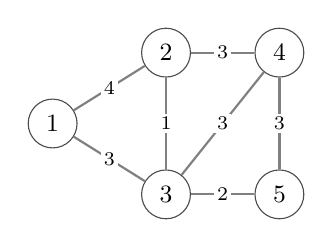
\begin{tikzpicture}[x=0.9cm, y=0.9cm]
\node[mst-v] (v1) at (0,1) {$1$};
\node[mst-v] (v2) at (1.6,2) {$2$};
\node[mst-v] (v3) at (1.6,0) {$3$};
\node[mst-v] (v4) at (3.2,2) {$4$};
\node[mst-v] (v5) at (3.2,0) {$5$};
\draw[mst-e] (v1) -- node[mst-w] {4} (v2);
\draw[mst-e] (v1) -- node[mst-w] {3} (v3);
\draw[mst-e] (v2) -- node[mst-w] {1} (v3);
\draw[mst-e] (v2) -- node[mst-w] {3} (v4);
\draw[mst-e] (v3) -- node[mst-w] {3} (v4);
\draw[mst-e] (v3) -- node[mst-w] {2} (v5);
\draw[mst-e] (v4) -- node[mst-w] {3} (v5);
\end{tikzpicture}
&
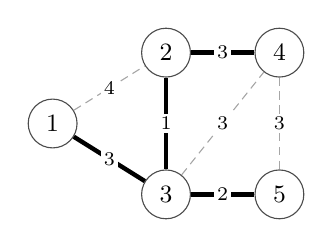
\begin{tikzpicture}[x=0.9cm, y=0.9cm]
\node[mst-v] (v1) at (0,1) {$1$};
\node[mst-v] (v2) at (1.6,2) {$2$};
\node[mst-v] (v3) at (1.6,0) {$3$};
\node[mst-v] (v4) at (3.2,2) {$4$};
\node[mst-v] (v5) at (3.2,0) {$5$};
\draw[mst-x] (v1) -- node[mst-w] {4} (v2);
\draw[mst-t] (v1) -- node[mst-w] {3} (v3);
\draw[mst-t] (v2) -- node[mst-w] {1} (v3);
\draw[mst-t] (v2) -- node[mst-w] {3} (v4);
\draw[mst-x] (v3) -- node[mst-w] {3} (v4);
\draw[mst-t] (v3) -- node[mst-w] {2} (v5);
\draw[mst-x] (v4) -- node[mst-w] {3} (v5);
\end{tikzpicture}
&
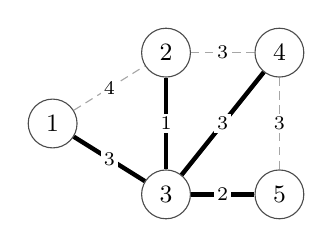
\begin{tikzpicture}[x=0.9cm, y=0.9cm]
\node[mst-v] (v1) at (0,1) {$1$};
\node[mst-v] (v2) at (1.6,2) {$2$};
\node[mst-v] (v3) at (1.6,0) {$3$};
\node[mst-v] (v4) at (3.2,2) {$4$};
\node[mst-v] (v5) at (3.2,0) {$5$};
\draw[mst-x] (v1) -- node[mst-w] {4} (v2);
\draw[mst-t] (v1) -- node[mst-w] {3} (v3);
\draw[mst-t] (v2) -- node[mst-w] {1} (v3);
\draw[mst-x] (v2) -- node[mst-w] {3} (v4);
\draw[mst-t] (v3) -- node[mst-w] {3} (v4);
\draw[mst-t] (v3) -- node[mst-w] {2} (v5);
\draw[mst-x] (v4) -- node[mst-w] {3} (v5);
\end{tikzpicture}
\\
\small 原圖 & \small Kruskal（照 $\prec$） & \small Prim（從 $1$ 開始）
\end{tabular}
\diagcaption{平手時兩個演算法選出不同的最小生成樹。 頂點 $4$ 一定要從三條權重 $3$ 的邊
$2$--$4$、$3$--$4$、$4$--$5$ 裡挑一條接進來，三種挑法都是最小生成樹。}
\label{fig:mst-ties}
\end{center}

Kruskal 照 $\prec$ 排序：$2$--$3$（$1$）、$3$--$5$（$2$），接著四條權重 $3$ 的邊依小端點、
大端點排成 $1$--$3$、$2$--$4$、$3$--$4$、$4$--$5$。 $1$--$3$ 和 $2$--$4$ 都選，這時已經
選滿 $4$ 條。 Prim 從 $1$ 開始：先取出 $3$（$\mathit{key} = 3$），$3$ 把 $\mathit{key}[2]$
改成 $1$、$\mathit{key}[4]$ 改成 $3$（$\pi[4] = 3$）、$\mathit{key}[5]$ 改成 $2$；接著取出 $2$，
邊 $2$--$4$ 的權重 $3$ 沒有\textbf{小於} $\mathit{key}[4] = 3$，不更新；再取出 $5$，$4$--$5$ 也一
樣；最後 $4$ 經由 $\pi[4] = 3$ 接進來。 兩棵樹差在頂點 $4$ 接在哪裡，都對。

這說明了兩件事。 第一，Prim 的平手規則比的是頂點，不是邊，所以它的結果不一定是引
理~\ref{lem:mst-ties} 的 $T_{\prec}$；它仍然是最小生成樹，因為定理~\ref{thm:mst-prim} 的證明
只用到「輕邊之一」。 第二，第 10 行如果改成 $\le$，$\pi[4]$ 會被後來一樣輕的邊換掉，最後變成
$4$--$5$，又是另一棵。 所以答案不只一個時，平手規則（包括更新時用 $<$ 還是 $\le$）一定要
照題目。

\subsection{C 程式}

下面兩個程式都從頂點 $1$ 開始，印出每回合加入的頂點和邊。 第一個照
虛擬碼~\ref{alg:mst-prim}，用鄰接串列和第~8~章的帶索引最小堆積，另外數
\proc{Decrease-Key} 做了幾次；第二個照虛擬碼~\ref{alg:mst-prim-array}，用鄰接矩陣。 兩
個程式的平手規則相同，對同一張圖印出的過程應該完全相同。

\begin{cbookrecap}[第~14~章結構、第~19~章 \texttt{malloc} 與鏈結串列]
堆積的三個陣列包在 \texttt{MinHeap} 結構裡：\texttt{heap[i]} 是第 \texttt{i} 格放的頂點，
\texttt{pos[v]} 是頂點 \texttt{v} 在哪一格，\texttt{key[v]} 是它的鍵。 交換兩格時兩個頂點的
\texttt{pos} 都要改，寫成 \texttt{swap\_at}；這和第~8~章急診室候診名單的程式是同一個寫
法。 函式收到的是 \texttt{MinHeap *h}，用 \texttt{h->key[v]} 存取，改的是呼叫端那一份。
\end{cbookrecap}

\begin{example}[label=ex:mst-prim-heap]{c}{(prim\_heap.c) Prim 演算法：鄰接串列加帶索引最小堆積}
#include <stdio.h>
#include <stdlib.h>
#include <limits.h>

typedef struct Node {
    int v, w;
    struct Node *next;
} Node;

typedef struct {
    int n;
    Node **adj;     // adj[u]：u 的鄰居，編號由小到大
} Graph;

// 把 v 插進 adj[u]，保持由小到大
int add_arc(Graph *g, int u, int v, int w)
{
    Node *x = malloc(sizeof *x);
    if (x == NULL) {
        return 0;
    }
    Node **p = &g->adj[u];
    while (*p != NULL && (*p)->v < v) {
        p = &(*p)->next;
    }
    x->v = v;
    x->w = w;
    x->next = *p;
    *p = x;
    return 1;
}

void free_graph(Graph *g)
{
    for (int u = 0; g->adj != NULL && u < g->n; u++) {
        Node *x = g->adj[u];
        while (x != NULL) {
            Node *next = x->next;
            free(x);
            x = next;
        }
    }
    free(g->adj);
}

// 第 8 章的帶索引最小堆積。 比較的鍵是 (key, 頂點編號)，
// 所以 key 相同時編號小的先出來。
typedef struct {
    int *heap;      // heap[0..size-1]：頂點編號
    int *pos;       // pos[v]：v 在 heap 的哪一格，-1 表示已經取出
    long long *key;
    int size;
} MinHeap;

static int before(const MinHeap *h, int u, int v)
{
    return h->key[u] < h->key[v] || (h->key[u] == h->key[v] && u < v);
}

static void swap_at(MinHeap *h, int i, int j)
{
    int u = h->heap[i], v = h->heap[j];
    h->heap[i] = v;
    h->heap[j] = u;
    h->pos[v] = i;
    h->pos[u] = j;
}

static void sift_up(MinHeap *h, int i)
{
    while (i > 0 && before(h, h->heap[i], h->heap[(i - 1) / 2])) {
        swap_at(h, i, (i - 1) / 2);
        i = (i - 1) / 2;
    }
}

static void sift_down(MinHeap *h, int i)
{
    for (;;) {
        int j = 2 * i + 1;
        if (j >= h->size) {
            return;
        }
        if (j + 1 < h->size && before(h, h->heap[j + 1], h->heap[j])) {
            j++;
        }
        if (!before(h, h->heap[j], h->heap[i])) {
            return;
        }
        swap_at(h, i, j);
        i = j;
    }
}

int extract_min(MinHeap *h)
{
    int u = h->heap[0];
    swap_at(h, 0, h->size - 1);
    h->size--;
    h->pos[u] = -1;
    sift_down(h, 0);
    return u;
}

void decrease_key(MinHeap *h, int v, long long k)
{
    h->key[v] = k;
    sift_up(h, h->pos[v]);
}

int main(void)
{
    int n, m;
    if (scanf("%d %d", &n, &m) != 2 || n <= 0 || m < 0) {
        return 1;
    }
    Graph g = {n, calloc(n, sizeof(Node *))};
    MinHeap h = {malloc(n * sizeof(int)), malloc(n * sizeof(int)),
                 malloc(n * sizeof(long long)), n};
    int *pi = malloc(n * sizeof(int));
    int ok = g.adj != NULL && h.heap != NULL && h.pos != NULL
             && h.key != NULL && pi != NULL;
    for (int i = 0; ok && i < m; i++) {
        int u, v, w;
        ok = scanf("%d %d %d", &u, &v, &w) == 3 && u >= 1 && u <= n
             && v >= 1 && v <= n;
        if (ok && u != v) {     // 自環不會在生成樹裡，直接丟掉
            ok = add_arc(&g, u - 1, v - 1, w) && add_arc(&g, v - 1, u - 1, w);
        }
    }
    if (ok) {
        // 所有頂點一開始都在堆積裡，key 是無限大；起點是頂點 1
        for (int v = 0; v < n; v++) {
            h.heap[v] = v;
            h.pos[v] = v;
            h.key[v] = LLONG_MAX;
            pi[v] = -1;
        }
        h.key[0] = 0;
        long long total = 0;
        int calls = 0, added = 0;
        while (h.size > 0) {
            int u = extract_min(&h);
            if (h.key[u] == LLONG_MAX) {
                break;                      // 剩下的頂點都連不到
            }
            added++;
            if (pi[u] < 0) {
                printf("add %d\n", u + 1);
            } else {
                printf("add %d via %d-%d (%lld)\n", u + 1, pi[u] + 1, u + 1, h.key[u]);
                total += h.key[u];
            }
            for (Node *x = g.adj[u]; x != NULL; x = x->next) {
                int v = x->v;
                if (h.pos[v] >= 0 && x->w < h.key[v]) {
                    pi[v] = u;
                    decrease_key(&h, v, x->w);
                    calls++;
                }
            }
        }
        printf("decrease-key calls %d\n", calls);
        if (added == n) {
            printf("MST weight %lld\n", total);
        } else {
            printf("not connected: reached %d of %d vertices\n", added, n);
        }
    }
    free_graph(&g);
    free(h.heap);
    free(h.pos);
    free(h.key);
    free(pi);
    return ok ? 0 : 1;
}
\end{example}
\iosample{8 13 \\ 1 2 7 \\ 2 3 12 \\ 3 4 14 \\ 5 6 9 \\ 6 7 4 \\ 7 8 13 \\ 1 5 1 \\ 2 6 6 \\ 3 7 11 \\ 4 8 3 \\ 1 6 10 \\ 2 7 5 \\ 3 8 8}{add 1 \\ add 5 via 1-5 (1) \\ add 2 via 1-2 (7) \\ add 7 via 2-7 (5) \\ add 6 via 7-6 (4) \\ add 3 via 7-3 (11) \\ add 8 via 3-8 (8) \\ add 4 via 8-4 (3) \\ decrease-key calls 13 \\ MST weight 39}

一開始所有 $\mathit{key}$ 都是 \texttt{LLONG\_MAX}，只有頂點 $0$（書上的 $1$）是 $0$，陣列
\texttt{heap} 照編號排就已經是一個合法的堆積，不用另外建。 \texttt{pos[v] >= 0} 就是虛擬
碼的「$v$ 還在 $Q$ 裡」。 自環在讀入時就丟掉；平行邊不用特別處理，比較輕的那條自然會讓
$\mathit{key}$ 變得比較小。

\begin{example}[label=ex:mst-prim-array]{c}{(prim\_array.c) Prim 演算法：鄰接矩陣、$O(n^2)$}
#include <stdio.h>
#include <stdlib.h>
#include <limits.h>

#define NO_EDGE INT_MAX     // 鄰接矩陣裡「沒有邊」，也當作 key 的無限大

int main(void)
{
    int n, m;
    if (scanf("%d %d", &n, &m) != 2 || n <= 0 || m < 0) {
        return 1;
    }
    int *W = malloc((size_t)n * n * sizeof(int));  // W[u * n + v]
    int *key = malloc(n * sizeof(int));
    int *pi = malloc(n * sizeof(int));
    int *in_tree = calloc(n, sizeof(int));
    int ok = W != NULL && key != NULL && pi != NULL && in_tree != NULL;
    for (int i = 0; ok && i < n * n; i++) {
        W[i] = NO_EDGE;
    }
    for (int i = 0; ok && i < m; i++) {
        int u, v, w;
        ok = scanf("%d %d %d", &u, &v, &w) == 3 && u >= 1 && u <= n
             && v >= 1 && v <= n && w < NO_EDGE;
        if (ok && u != v && w < W[(u - 1) * n + (v - 1)]) {
            W[(u - 1) * n + (v - 1)] = w;   // 平行邊只留最輕的
            W[(v - 1) * n + (u - 1)] = w;
        }
    }
    if (ok) {
        for (int v = 0; v < n; v++) {
            key[v] = NO_EDGE;
            pi[v] = -1;
        }
        key[0] = 0;
        long long total = 0;
        int added = 0;
        for (int i = 0; i < n; i++) {
            int u = -1;
            for (int v = 0; v < n; v++) {   // 找 key 最小的；平手時編號小的
                if (!in_tree[v] && (u < 0 || key[v] < key[u])) {
                    u = v;
                }
            }
            if (key[u] == NO_EDGE) {
                break;                      // 剩下的頂點都連不到
            }
            in_tree[u] = 1;
            added++;
            if (pi[u] < 0) {
                printf("add %d\n", u + 1);
            } else {
                printf("add %d via %d-%d (%d)\n", u + 1, pi[u] + 1, u + 1, key[u]);
                total += key[u];
            }
            for (int v = 0; v < n; v++) {
                if (!in_tree[v] && W[u * n + v] < key[v]) {
                    key[v] = W[u * n + v];
                    pi[v] = u;
                }
            }
        }
        if (added == n) {
            printf("MST weight %lld\n", total);
        } else {
            printf("not connected: reached %d of %d vertices\n", added, n);
        }
    }
    free(W);
    free(key);
    free(pi);
    free(in_tree);
    return ok ? 0 : 1;
}
\end{example}
\iosample{8 13 \\ 1 2 7 \\ 2 3 12 \\ 3 4 14 \\ 5 6 9 \\ 6 7 4 \\ 7 8 13 \\ 1 5 1 \\ 2 6 6 \\ 3 7 11 \\ 4 8 3 \\ 1 6 10 \\ 2 7 5 \\ 3 8 8}{add 1 \\ add 5 via 1-5 (1) \\ add 2 via 1-2 (7) \\ add 7 via 2-7 (5) \\ add 6 via 7-6 (4) \\ add 3 via 7-3 (11) \\ add 8 via 3-8 (8) \\ add 4 via 8-4 (3) \\ MST weight 39}

鄰接矩陣用一維陣列存，第 $u$ 列第 $v$ 行放在 \texttt{W[u * n + v]}，只要一次
\texttt{malloc}。 配置大小先轉成 \texttt{size\_t} 再乘，避免 $n$ 很大時 \texttt{int} 溢位。
\texttt{INT\_MAX} 同時代表「沒有邊」和 $\infty$：沒有邊的格子永遠不會小於 $\mathit{key}$，
更新 $\mathit{key}$ 的迴圈自然跳過它。 這個程式不需要堆積，整個程式不到八十行，$n$ 幾千、
邊很密的時候反而是最快的寫法。

\section{Sollin 演算法（Borůvka 演算法）}
\label{sec:mst-sollin}

Kruskal 和 Prim 每一步只加一條邊。 Sollin 演算法一次加很多條：把目前森林裡的每一棵樹看
成一個\textbf{元件}，每個元件同時挑一條「連到別的元件的最輕的邊」，全部加進來，元件就兩
兩併起來。 重複幾回合，直到只剩一個元件。 這個方法最早是 Borůvka 在 1926 年為了規劃電網
提出的，後來又被好幾個人重新發現，不少資料結構課本叫它 Sollin 演算法。

每個元件 $C$ 挑的邊，是切割 $(C, V - C)$ 的輕邊。 切割尊重目前的森林（森林的邊不會一端在
$C$ 裡、一端在外面），所以由切割性質，\textbf{單獨看}每一條都是安全的。 麻煩在「同時」：
定理~\ref{thm:mst-cut} 一次只保證一條。 下面會看到，權重相同時如果每個元件各挑各的，一次加
進來的邊可能形成環。

\begin{pseudo}[label=alg:mst-sollin]{Sollin 演算法}
\Procedure{MST-Sollin}{$G, w$}
    \State $A \gets \emptyset$
    \For{每個頂點 $v \in G.V$}
        \State \Call{Make-Set}{$v$}
    \EndFor
    \While{$|A| < n - 1$}
        \For{每個頂點 $v \in G.V$}
            \State $\mathit{cheap}[v] \gets \NIL$
        \EndFor
        \For{每條邊 $e = (u, v) \in G.E$}
            \State $a \gets \Call{Find-Set}{u}$；$b \gets \Call{Find-Set}{v}$
            \If{$a \ne b$}
                \If{$\mathit{cheap}[a] = \NIL$ \OR $e \prec \mathit{cheap}[a]$}
                    \State $\mathit{cheap}[a] \gets e$
                \EndIf
                \If{$\mathit{cheap}[b] = \NIL$ \OR $e \prec \mathit{cheap}[b]$}
                    \State $\mathit{cheap}[b] \gets e$
                \EndIf
            \EndIf
        \EndFor
        \For{每個 $\mathit{cheap}[c] \ne \NIL$ 的 $c$}
            \State $(u, v) \gets \mathit{cheap}[c]$
            \If{$\Call{Find-Set}{u} \ne \Call{Find-Set}{v}$} \Comment{兩個元件可能挑到同一條}
                \State $A \gets A \cup \{(u, v)\}$；\Call{Union}{$u, v$}
            \EndIf
        \EndFor
    \EndWhile
    \State \Return $A$
\EndProcedure
\end{pseudo}

$\mathit{cheap}[c]$ 用元件的代表 $c$ 當索引，記這個元件目前找到最輕的往外的邊。 第 8--14
行掃一遍所有的邊，每條跨越兩個元件的邊，兩端的元件各拿它比一次；比較一律用
第~\ref{sec:mst-ties}~節的 $\prec$。 第 15--18 行把挑到的邊加進來。 同一條邊常常被兩端的
元件同時挑中（例如兩個元件互相是對方最近的），第二次處理時兩端已經合併，第 17 行把它跳
過。 圖不連通時第 5 行的條件永遠不會成立，實作時要改成「這一回合沒有加任何邊就停」，結果
是最小生成森林。

\subsection{回合數}

\begin{theorem}
\label{thm:mst-rounds}
$G$ 連通時，Sollin 演算法每一回合至少讓元件數減半，所以最多 $\lfloor \lg n \rfloor$ 回合。
\end{theorem}

\begin{proof}
設某回合開始時有 $k \ge 2$ 個元件。 $G$ 連通，每個元件都有往外的邊，都會挑到一條，這條邊
把它和另一個元件連起來。 所以這一回合結束時，每個新的元件都至少包含兩個舊的元件，新的
元件數 $\le \lfloor k/2 \rfloor$。 從 $n$ 個元件開始，$r$ 回合後最多剩 $\lfloor n / 2^r
\rfloor$ 個（每回合都無條件捨去），$r = \lfloor \lg n \rfloor$ 時這個數是 $1$。
\end{proof}

每一回合第 6--7 行是 $\Theta(n)$，第 8--14 行對每條邊做兩次 \proc{Find-Set}，第 15--18 行
最多 $n$ 次，用第~13~章的互斥集合是 $O((n + m)\,\alpha(n))$。 也可以每回合開始時用第~21~章
的 DFS 把森林的元件重新編號，不用互斥集合，每回合 $\Theta(n + m)$。 總時間 $O(m \lg n)$，
和另外兩個演算法同級。 它的好處是每一回合裡各個元件的工作互不相干，很適合分給很多處理器
同時做；而且回合數少，每回合結束時把元件縮成一個點、重複的邊只留最輕的，圖會越縮越小。
Karger、Klein、Tarjan 的線性期望時間演算法（見延伸閱讀）就用 Sollin 的回合當成基本步驟。

\subsection{平手時要用一致的規則}

看一個三角形：三個頂點 $1, 2, 3$，三條邊的權重都是 $5$。 第一回合每個頂點自己是一個元件，
每個都要挑一條最輕的往外的邊，而每個頂點的兩條邊一樣輕。 如果各自隨便挑，可能出現
「$1$ 挑 $1$--$2$、$2$ 挑 $2$--$3$、$3$ 挑 $3$--$1$」：每一條單獨看都是輕邊，但三條一起加
進來是一個環。

\begin{center}
\begin{tabular}{cc}
\begin{tikzpicture}[x=1.2cm, y=1.2cm]
\node[mst-v] (a) at (0,0) {$1$};
\node[mst-v] (b) at (2,0) {$2$};
\node[mst-v] (c) at (1,1.6) {$3$};
\draw[mst-new] (a) -- node[mst-w] (ab) {5} (b);
\draw[mst-new] (b) -- node[mst-w] (bc) {5} (c);
\draw[mst-new] (c) -- node[mst-w] (ca) {5} (a);
\draw[mst-pick] (a) to[bend right=25] (ab);
\draw[mst-pick] (b) to[bend right=25] (bc);
\draw[mst-pick] (c) to[bend right=25] (ca);
\end{tikzpicture}
&
\begin{tikzpicture}[x=1.2cm, y=1.2cm]
\node[mst-v] (a) at (0,0) {$1$};
\node[mst-v] (b) at (2,0) {$2$};
\node[mst-v] (c) at (1,1.6) {$3$};
\draw[mst-t] (a) -- node[mst-w] (ab) {5} (b);
\draw[mst-x] (b) -- node[mst-w] (bc) {5} (c);
\draw[mst-t] (c) -- node[mst-w] (ca) {5} (a);
\draw[mst-pick] (a) to[bend right=25] (ab);
\draw[mst-pick] (b) to[bend left=25] (ab);
\draw[mst-pick] (c) to[bend left=25] (ca);
\end{tikzpicture}
\\
\small 各挑各的：三條邊形成環 & \small 照 $\prec$：$1$、$2$ 都挑 $1$--$2$，$3$ 挑 $1$--$3$
\end{tabular}
\diagcaption{三條邊權重相同的三角形。 箭頭從頂點指向它在第一回合挑的邊。}
\label{fig:mst-sollin-cycle}
\end{center}

照 $\prec$ 比較時，頂點 $1$ 的兩條邊 $(5, 1, 2) \prec (5, 1, 3)$，挑 $1$--$2$；頂點 $2$ 的兩
條邊 $(5, 1, 2) \prec (5, 2, 3)$，也挑 $1$--$2$；頂點 $3$ 的兩條邊 $(5, 1, 3) \prec (5, 2,
3)$，挑 $1$--$3$。 加進來的是 $1$--$2$ 和 $1$--$3$，沒有環。 一般的情形是下面的定理：

\begin{theorem}
\label{thm:mst-sollin}
如果所有元件挑邊時都照同一個嚴格的全序 $\prec$（第~\ref{sec:mst-ties}~節）比較，Sollin 演
算法每一回合挑到的邊加起來不會形成環，最後得到的是引理~\ref{lem:mst-ties} 的 $T_{\prec}$，也
就是一棵最小生成樹。
\end{theorem}

\begin{proof}
由引理~\ref{lem:mst-ties}，照 $\prec$ 比較等於在權重互不相同的 $w'$ 上比較，$w'$ 的最小生
成樹只有 $T_{\prec}$ 一棵。 對回合做歸納，假設回合開始時 $A \subseteq T_{\prec}$（一開始
$A = \emptyset$）。 這一回合元件 $C$ 挑的邊 $e_C$，是切割 $(C, V - C)$ 在 $w'$ 之下唯一的輕
邊，由系理~\ref{cor:mst-cut-strict}，$e_C$ 在 $w'$ 的每一棵最小生成樹裡，也就是 $e_C \in
T_{\prec}$。 所以 $A$ 加上這一回合所有挑到的邊，仍然包含在 $T_{\prec}$ 裡，而 $T_{\prec}$
是樹，這些邊不會形成環。 最後 $A$ 有 $n - 1$ 條邊，就是 $T_{\prec}$。
\end{proof}

證明的關鍵是「每個元件挑的邊都在\textbf{同一棵}樹 $T_{\prec}$ 裡」。 各挑各的時候，每條邊
雖然各自屬於某一棵最小生成樹，卻可能屬於不同的那一棵，合起來就不保證了。

虛擬碼~\ref{alg:mst-sollin} 第 17 行的檢查，在程式裡其實也會把形成環的邊擋掉。 但手算時
習慣把整回合挑到的邊一次畫上去，平手規則不一致就會畫出環；更重要的是，上面的正確性證明
要靠一致的 $\prec$。 所以寫 Sollin 演算法時，不管手算還是程式，平手規則都要先定好、全部
元件共用。

\subsection{手算追蹤}

露營區的權重互不相同，不會遇到平手。 第一回合每個頂點自己是一個元件：

\begin{center}
\small
\begin{tabular}{cccccccc}
\toprule
$\{1\}$ & $\{2\}$ & $\{3\}$ & $\{4\}$ & $\{5\}$ & $\{6\}$ & $\{7\}$ & $\{8\}$ \\
\midrule
$1$--$5$（$1$） & $2$--$7$（$5$） & $3$--$8$（$8$） & $4$--$8$（$3$） & $1$--$5$（$1$） &
$6$--$7$（$4$） & $6$--$7$（$4$） & $4$--$8$（$3$） \\
\bottomrule
\end{tabular}
\end{center}

八個元件挑了八次，但 $1$--$5$、$6$--$7$、$4$--$8$ 各被挑了兩次，去掉重複後加入五條邊：
$1$--$5$、$2$--$7$、$3$--$8$、$4$--$8$、$6$--$7$。 元件剩下 $\{1, 5\}$、$\{2, 6, 7\}$、
$\{3, 4, 8\}$ 三個。

\begin{center}
\begin{tikzpicture}[x=1.2cm, y=1.2cm]
\node[mst-v] (v1) at (0,2) {$1$};
\node[mst-v] (v2) at (2,2) {$2$};
\node[mst-v] (v3) at (4,2) {$3$};
\node[mst-v] (v4) at (6,2) {$4$};
\node[mst-v] (v5) at (0,0) {$5$};
\node[mst-v] (v6) at (2,0) {$6$};
\node[mst-v] (v7) at (4,0) {$7$};
\node[mst-v] (v8) at (6,0) {$8$};
\begin{scope}[on background layer]
\draw[mst-hull] (v1.center) -- (v5.center);
\filldraw[mst-hull] (v2.center) -- (v7.center) -- (v6.center) -- cycle;
\filldraw[mst-hull] (v3.center) -- (v8.center) -- (v4.center) -- cycle;
\end{scope}
\draw[mst-new] (v1) -- node[mst-w] {7} (v2);
\draw[mst-x] (v2) -- node[mst-w] {12} (v3);
\draw[mst-x] (v3) -- node[mst-w] {14} (v4);
\draw[mst-x] (v5) -- node[mst-w] {9} (v6);
\draw[mst-t] (v6) -- node[mst-w] {4} (v7);
\draw[mst-x] (v7) -- node[mst-w] {13} (v8);
\draw[mst-t] (v1) -- node[mst-w] {1} (v5);
\draw[mst-x] (v2) -- node[mst-w] {6} (v6);
\draw[mst-new] (v3) -- node[mst-w] {11} (v7);
\draw[mst-t] (v4) -- node[mst-w] {3} (v8);
\draw[mst-x] (v1) -- node[mst-w] {10} (v6);
\draw[mst-t] (v2) -- node[mst-w] {5} (v7);
\draw[mst-t] (v3) -- node[mst-w] {8} (v8);
\end{tikzpicture}
\diagcaption{第一回合後的三個元件（藍底），粗黑線是第一回合加入的五條邊。 紅線是第二回合
加入的兩條，虛線是始終沒選的邊。}
\label{fig:mst-sollin}
\end{center}

第二回合，三個元件往外的邊：

\begin{center}
\small
\begin{tabular}{lll}
\toprule
元件 & 往外的邊（權重） & 挑 \\
\midrule
$\{1, 5\}$ & $1$--$2$（$7$）、$5$--$6$（$9$）、$1$--$6$（$10$） & $1$--$2$（$7$） \\
$\{2, 6, 7\}$ & $1$--$2$（$7$）、$5$--$6$（$9$）、$1$--$6$（$10$）、$3$--$7$（$11$）、$2$--$3$（$12$）、$7$--$8$（$13$） & $1$--$2$（$7$） \\
$\{3, 4, 8\}$ & $3$--$7$（$11$）、$2$--$3$（$12$）、$7$--$8$（$13$） & $3$--$7$（$11$） \\
\bottomrule
\end{tabular}
\end{center}

$\{1, 5\}$ 和 $\{2, 6, 7\}$ 都挑 $1$--$2$，加入 $1$--$2$、$3$--$7$ 兩條，只剩一個元件，結束。 兩
回合，總共 $7$ 條邊、總權重 $39$，和前兩節的結果相同。 $n = 8$ 時定理~\ref{thm:mst-rounds}
的上限是 $3$ 回合，這張圖兩回合就做完了。

\subsection{C 程式}

下面的程式照虛擬碼~\ref{alg:mst-sollin} 執行，每回合先依元件裡最小的頂點編號，印出每個元
件和它挑的邊，再印出這一回合真的加入的邊。 為了印出元件的成員，程式每次都重新掃一遍所
有頂點，$O(n^2)$，只是為了輸出好看；演算法本身不需要。 互斥集合只用路徑壓縮，因為這裡
的重點是挑邊。

\begin{example}[label=ex:mst-sollin]{c}{(sollin.c) Sollin 演算法：每個元件同時挑最輕的往外的邊}
#include <stdio.h>
#include <stdlib.h>

typedef struct {
    int u, v, w;    // 讀入時讓 u < v
} Edge;

// 一致的平手規則：先比權重，再比小端點，再比大端點
int lighter(const Edge *x, const Edge *y)
{
    if (x->w != y->w) {
        return x->w < y->w;
    }
    if (x->u != y->u) {
        return x->u < y->u;
    }
    return x->v < y->v;
}

int find_set(int *p, int x)
{
    int r = x;
    while (p[r] != r) {
        r = p[r];
    }
    while (p[x] != r) {
        int next = p[x];
        p[x] = r;
        x = next;
    }
    return r;
}

int main(void)
{
    int n, m;
    if (scanf("%d %d", &n, &m) != 2 || n <= 0 || m < 0) {
        return 1;
    }
    Edge *e = malloc((m > 0 ? m : 1) * sizeof *e);
    int *p = malloc(n * sizeof(int));
    int *cheap = malloc(n * sizeof(int));  // cheap[r]：根 r 的元件挑到的邊（索引）
    int ok = e != NULL && p != NULL && cheap != NULL;
    for (int i = 0; ok && i < m; i++) {
        int u, v, w;
        ok = scanf("%d %d %d", &u, &v, &w) == 3 && u >= 1 && u <= n
             && v >= 1 && v <= n;
        if (ok) {
            e[i].u = (u < v ? u : v) - 1;
            e[i].v = (u < v ? v : u) - 1;
            e[i].w = w;
        }
    }
    if (ok) {
        for (int x = 0; x < n; x++) {
            p[x] = x;
        }
        long long total = 0;
        int taken = 0, round = 0, progress = 1;
        while (taken < n - 1 && progress) {
            for (int x = 0; x < n; x++) {
                cheap[x] = -1;
            }
            // 每條邊兩端的元件各自比一次
            for (int i = 0; i < m; i++) {
                int a = find_set(p, e[i].u), b = find_set(p, e[i].v);
                if (a == b) {
                    continue;
                }
                if (cheap[a] < 0 || lighter(&e[i], &e[cheap[a]])) {
                    cheap[a] = i;
                }
                if (cheap[b] < 0 || lighter(&e[i], &e[cheap[b]])) {
                    cheap[b] = i;
                }
            }
            printf("round %d\n", ++round);
            // 依元件裡最小的頂點編號，印出每個元件和它挑的邊
            for (int x = 0; x < n; x++) {
                int r = find_set(p, x);
                int first = 1;
                for (int y = 0; y < x && first; y++) {
                    first = find_set(p, y) != r;
                }
                if (!first || cheap[r] < 0) {
                    continue;
                }
                printf("{");
                for (int y = x, sep = 0; y < n; y++) {
                    if (find_set(p, y) == r) {
                        printf(sep++ ? ",%d" : "%d", y + 1);
                    }
                }
                const Edge *c = &e[cheap[r]];
                printf("} picks %d-%d (%d)\n", c->u + 1, c->v + 1, c->w);
            }
            // 把挑到的邊加進來；兩個元件挑到同一條時，第二次會被略過
            progress = 0;
            printf("added:");
            for (int r = 0; r < n; r++) {
                if (cheap[r] < 0) {
                    continue;
                }
                const Edge *c = &e[cheap[r]];
                int a = find_set(p, c->u), b = find_set(p, c->v);
                if (a != b) {
                    p[b] = a;
                    total += c->w;
                    taken++;
                    progress = 1;
                    printf(" %d-%d", c->u + 1, c->v + 1);
                }
            }
            printf("\n");
        }
        if (taken == n - 1) {
            printf("MST weight %lld, %d edges\n", total, taken);
        } else {
            printf("not connected: forest weight %lld, %d edges\n", total, taken);
        }
    }
    free(e);
    free(p);
    free(cheap);
    return ok ? 0 : 1;
}
\end{example}
\iosample{8 13 \\ 1 2 7 \\ 2 3 12 \\ 3 4 14 \\ 5 6 9 \\ 6 7 4 \\ 7 8 13 \\ 1 5 1 \\ 2 6 6 \\ 3 7 11 \\ 4 8 3 \\ 1 6 10 \\ 2 7 5 \\ 3 8 8}{round 1 \\ \{1\} picks 1-5 (1) \\ \{2\} picks 2-7 (5) \\ \{3\} picks 3-8 (8) \\ \{4\} picks 4-8 (3) \\ \{5\} picks 1-5 (1) \\ \{6\} picks 6-7 (4) \\ \{7\} picks 6-7 (4) \\ \{8\} picks 4-8 (3) \\ added: 1-5 2-7 3-8 4-8 6-7 \\ round 2 \\ \{1,5\} picks 1-2 (7) \\ \{2,6,7\} picks 1-2 (7) \\ \{3,4,8\} picks 3-7 (11) \\ added: 1-2 3-7 \\ MST weight 39, 7 edges}

\texttt{cheap} 以每回合開始時的根當索引；加邊時元件會合併、根會改變，但 \texttt{cheap} 記
的是邊的索引，加邊前重新 \texttt{find\_set} 檢查兩端，所以不受影響。 \texttt{progress} 處
理圖不連通的情形：某一回合沒有任何元件挑得到邊，就停下來，印出最小生成森林的權重。
如果比較只看權重，每個元件留下的是它最先看到的那條，挑到哪一條會隨邊的輸入順序改變，手
算的答案就可能對不上。

\section{判定、次小生成樹、瓶頸與最短路徑樹}
\label{sec:mst-more}

這一節整理幾個常和最小生成樹一起考的觀念。 下面 $T$ 是一棵生成樹；對任兩個頂點 $x$、$y$，
$T$ 裡 $x$ 到 $y$ 恰好有一條簡單路徑，記成 $P_T(x, y)$，路徑上最重的邊的權重記成
$\mathit{max}_T(x, y)$。

\subsection{怎麼判斷一棵生成樹是不是最小的}

\begin{theorem}
\label{thm:mst-check}
生成樹 $T$ 是最小生成樹，若且唯若每一條不在 $T$ 裡的邊 $(x, y)$ 都滿足
\[
w(x, y) \ge \mathit{max}_T(x, y),
\]
也就是說，把任何一條非樹邊加進 $T$ 形成的環上，這條非樹邊是最重的（可以平手）。
\end{theorem}

\begin{proof}[$\Rightarrow$ 的證明]
假設某條非樹邊 $(x, y)$ 的權重小於 $P_T(x, y)$ 上某條邊 $f$。 把 $(x, y)$ 加進 $T$、拿掉 $f$：
$f$ 在 $x$ 到 $y$ 的路徑上，拿掉後 $x$、$y$ 分在兩塊，$(x, y)$ 把兩塊接回來，得到一棵生成
樹，總權重比 $w(T)$ 小，$T$ 就不是最小的。
\end{proof}

\begin{whybox}[定理~\ref{thm:mst-check} 的 $\Leftarrow$]
設 $T$ 滿足條件。 在所有最小生成樹裡，取一棵和 $T$ 共同的邊最多的，叫它 $T^*$。 如果 $T^* =
T$ 就證完了。 否則兩棵樹邊數一樣，$T^*$ 有一條不在 $T$ 裡的邊 $f = (x, y)$。

從 $T^*$ 拿掉 $f$，分成兩塊，$x$、$y$ 各在一塊。 $T$ 的路徑 $P_T(x, y)$ 從 $x$ 走到 $y$，一
定有一條邊 $e$ 跨越這兩塊。 $e$ 不是 $f$（$f$ 不在 $T$ 裡），而 $T^*$ 跨越這兩塊的邊只有 $f$，
所以 $e \notin T^*$。 由條件，$w(f) \ge \mathit{max}_T(x, y) \ge w(e)$。

令 $T'' = T^* - \{f\} \cup \{e\}$，它是生成樹，$w(T'') = w(T^*) - w(f) + w(e) \le w(T^*)$，所
以也是最小生成樹。 但 $T''$ 比 $T^*$ 多了一條和 $T$ 共同的邊 $e$（$f$ 本來就不是共同的），
和 $T^*$ 的取法矛盾。 所以 $T^* = T$，$T$ 是最小生成樹。
\end{whybox}

用這個定理檢查一棵樹，要知道每一對 $(x, y)$ 的 $\mathit{max}_T(x, y)$。 從每個頂點在 $T$ 上
做一次 BFS 或 DFS，沿路記下「到目前為止最重的邊」，一次 $\Theta(n)$，$n$ 次就把所有配對算
完，$\Theta(n^2)$；再掃一遍所有非樹邊，總共 $\Theta(n^2 + m)$。

在露營區驗證一下。 六條非樹邊各自形成的環：

\begin{center}
\small
\begin{tabular}{clcc}
\toprule
非樹邊 & $T$ 上的路徑 & 路徑上最重的邊 & 換進來的總權重 \\
\midrule
$2$--$6$（$6$） & $2, 7, 6$ & $2$--$7$（$5$） & $39 + 6 - 5 = 40$ \\
$5$--$6$（$9$） & $5, 1, 2, 7, 6$ & $1$--$2$（$7$） & $39 + 9 - 7 = 41$ \\
$1$--$6$（$10$） & $1, 2, 7, 6$ & $1$--$2$（$7$） & $39 + 10 - 7 = 42$ \\
$2$--$3$（$12$） & $2, 7, 3$ & $3$--$7$（$11$） & $39 + 12 - 11 = 40$ \\
$7$--$8$（$13$） & $7, 3, 8$ & $3$--$7$（$11$） & $39 + 13 - 11 = 41$ \\
$3$--$4$（$14$） & $3, 8, 4$ & $3$--$8$（$8$） & $39 + 14 - 8 = 45$ \\
\bottomrule
\end{tabular}
\end{center}

每一條非樹邊都比它的環上其他的邊重，所以 $T$ 是最小生成樹；而且都是\textbf{嚴格}比較重。
這也可以用來判斷最小生成樹是不是唯一（觀念題第~\ref{q:mst-unique-iff}~題）：

\begin{corollary}
\label{cor:mst-unique-iff}
最小生成樹 $T$ 是唯一的最小生成樹，若且唯若每一條非樹邊 $(x, y)$ 都滿足 $w(x, y) >
\mathit{max}_T(x, y)$。
\end{corollary}

\subsection{次小生成樹（觀念）}
\label{sec:mst-second}

\textbf{次小生成樹}（second-best minimum spanning tree）是除了最小生成樹以外，總權重最小
的生成樹。 上表最後一欄就是「換一條邊」得到的生成樹的總權重：把非樹邊 $(x, y)$ 換進來，同
時拿掉它的環上最重的樹邊，比拿掉環上其他樹邊都划算。

\begin{theorem}
\label{thm:mst-second}
如果 $G$ 的權重互不相同，$T$ 是它唯一的最小生成樹，那麼有一棵次小生成樹和 $T$ 只差一條
邊：它是 $T - \{f\} \cup \{(x, y)\}$，其中 $(x, y)$ 是某條非樹邊，$f$ 是 $P_T(x, y)$ 上最重的
邊。
\end{theorem}

證明用的也是換邊，這裡不證（CLRS 第 21 章章末的問題有完整的推導）。 由這個定理，求次小生
成樹的做法是：

\begin{enumerate}
\item 求出最小生成樹 $T$，$O(m \lg n)$。
\item 算出所有的 $\mathit{max}_T(x, y)$，$\Theta(n^2)$。
\item 對每一條非樹邊 $(x, y)$，算 $w(T) + w(x, y) - \mathit{max}_T(x, y)$，取最小的，$\Theta(m)$。
\end{enumerate}

露營區的次小生成樹總權重是 $40$，而且有兩棵：換進 $2$--$6$、拿掉 $2$--$7$，或換進
$2$--$3$、拿掉 $3$--$7$。 最小生成樹唯一，次小生成樹卻不一定唯一。

\begin{examnote}
「次小生成樹」有兩種定義，作答前先看題目用哪一種。 一種是「和最小生成樹不同的生成樹裡最
輕的」，最小生成樹不唯一時，它的權重就等於最小生成樹的權重；另一種是「總權重\textbf{嚴格
大於}最小生成樹的生成樹裡最輕的」。 用換邊法算第二種時，如果非樹邊和環上最重的樹邊一樣
重，要改拿環上嚴格比它輕的最重的邊。 另外，題目問「最小生成樹」和「最短路徑」的差別時，
常見的答法是舉一個小反例（下面的三角形），比長篇說明更有說服力。
\end{examnote}

\subsection{瓶頸：最小生成樹上的路徑讓最重的一段最輕}
\label{sec:mst-bottleneck}

一條路徑上最重的邊叫做它的\textbf{瓶頸}。 例如一輛貨車要從營地 $1$ 開到營地 $4$，每段路
有載重限制，它能載多重取決於路上限制最嚴的那一段。 把權重看成「需要的門檻」，問題就是：
在所有 $x$ 到 $y$ 的路徑裡，瓶頸最小是多少？ 最小生成樹直接給出答案。

\begin{theorem}
\label{thm:mst-bottleneck}
$T$ 是 $G$ 的一棵最小生成樹。 對任兩個頂點 $x \ne y$ 和 $G$ 裡任何一條 $x$ 到 $y$ 的路徑 $Q$，
$Q$ 上最重的邊至少是 $\mathit{max}_T(x, y)$。 也就是說，$T$ 上的路徑是瓶頸最小的路徑。
\end{theorem}

\begin{proof}
令 $e$ 是 $P_T(x, y)$ 上最重的邊。 從 $T$ 拿掉 $e$，分成兩塊，$x$、$y$ 各在一塊，令 $S$ 是 $x$
那一塊。 $e$ 一定是切割 $(S, V - S)$ 的輕邊：如果有一條跨越的邊 $f$ 比 $e$ 輕，$T - \{e\}
\cup \{f\}$ 就是更輕的生成樹。 路徑 $Q$ 從 $S$ 走到 $V - S$，至少經過一條跨越的邊 $f$，$w(f)
\ge w(e)$，所以 $Q$ 上最重的邊 $\ge w(e) = \mathit{max}_T(x, y)$。
\end{proof}

露營區裡 $1$ 到 $4$ 的樹上路徑是 $1, 2, 7, 3, 8, 4$，瓶頸是 $3$--$7$（$11$）。 任何一條從 $1$
到 $4$ 的路都要跨越切割 $(\{1, 2, 5, 6, 7\}, \{3, 4, 8\})$，跨越的邊是 $3$--$7$（$11$）、
$2$--$3$（$12$）、$7$--$8$（$13$），最輕也要 $11$。 實作時不一定要建出整棵樹：照 Kruskal 演
算法由輕到重加邊，$x$ 和 $y$ 第一次連通時加進來的那條邊，它的權重就是答案。

\subsection{最小生成樹不是最短路徑樹}
\label{sec:mst-spt}

從頂點 $r$ 出發，到每個頂點都走最短路徑（總權重最小的路徑），這些路徑合起來也是一棵生成
樹，叫做以 $r$ 為根的\textbf{最短路徑樹}，第~25~章的 Dijkstra 演算法會求它。 兩種樹都「讓
某個總和最小」，很容易混在一起，但它們最小化的東西不同：

\begin{itemize}
\item 最小生成樹讓\textbf{整棵樹的邊權重總和}最小，和根無關；
\item 最短路徑樹讓\textbf{從 $r$ 到每個頂點的路徑長度}各自最小，換一個根就可能換一棵樹。
\end{itemize}

\begin{center}
\begin{tabular}{ccc}
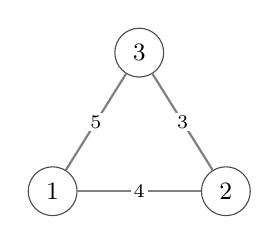
\begin{tikzpicture}[x=1.1cm, y=1.1cm]
\node[mst-v] (a) at (0,0) {$1$};
\node[mst-v] (b) at (2,0) {$2$};
\node[mst-v] (c) at (1,1.6) {$3$};
\draw[mst-e] (a) -- node[mst-w] {4} (b);
\draw[mst-e] (b) -- node[mst-w] {3} (c);
\draw[mst-e] (c) -- node[mst-w] {5} (a);
\end{tikzpicture}
&
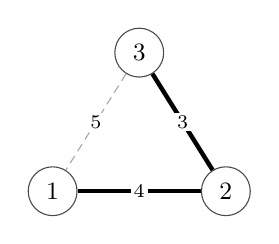
\begin{tikzpicture}[x=1.1cm, y=1.1cm]
\node[mst-v] (a) at (0,0) {$1$};
\node[mst-v] (b) at (2,0) {$2$};
\node[mst-v] (c) at (1,1.6) {$3$};
\draw[mst-t] (a) -- node[mst-w] {4} (b);
\draw[mst-t] (b) -- node[mst-w] {3} (c);
\draw[mst-x] (c) -- node[mst-w] {5} (a);
\end{tikzpicture}
&
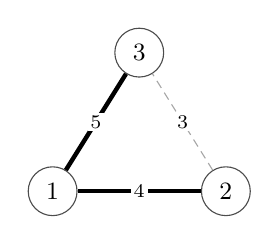
\begin{tikzpicture}[x=1.1cm, y=1.1cm]
\node[mst-v] (a) at (0,0) {$1$};
\node[mst-v] (b) at (2,0) {$2$};
\node[mst-v] (c) at (1,1.6) {$3$};
\draw[mst-t] (a) -- node[mst-w] {4} (b);
\draw[mst-x] (b) -- node[mst-w] {3} (c);
\draw[mst-t] (c) -- node[mst-w] {5} (a);
\end{tikzpicture}
\\
\small 原圖 & \small 最小生成樹，總權重 $7$ & \small 以 $1$ 為根的最短路徑樹，總權重 $9$
\end{tabular}
\diagcaption{最小生成樹和最短路徑樹不同的最小例子。 最小生成樹上 $1$ 到 $3$ 要走 $4 + 3 =
7$，最短路徑是直接走 $5$。}
\label{fig:mst-spt}
\end{center}

圖~\ref{fig:mst-spt} 是最小的反例：三角形的邊是 $3$、$4$、$5$。 最小生成樹丟掉最重的 $5$，
總權重 $7$；但從 $1$ 到 $3$，樹上要繞經 $2$ 走 $7$，直接走只要 $5$。 以 $1$ 為根的最短路徑
樹用 $1$--$2$ 和 $1$--$3$，總權重 $9$。 露營區也一樣：以 $1$ 為根的最短路徑樹有兩棵：$1$--$2$、
$1$--$5$、$2$--$3$、$2$--$7$、$7$--$8$、$8$--$4$ 這六條是共同的，頂點 $6$ 可以經由 $1$--$6$
或 $5$--$6$ 接進來（兩條路都是 $10$），總權重 $51$ 或 $50$，都比最小生成樹的 $39$ 重；反過來，最小生成樹上 $1$ 到 $4$ 要走 $7 + 5 + 11 + 8 + 3 = 34$，最短路徑只要 $28$。

幾個相關的事實，都可以直接從定義看出來：

\begin{itemize}
\item 最短路徑樹也是生成樹，所以它的總權重一定 $\ge$ 最小生成樹的總權重。
\item 每條邊的權重都加上同一個常數 $c$：每棵生成樹都恰好 $n - 1$ 條邊，總權重都加 $(n - 1)c$，
最小生成樹不變。 最短路徑則可能改變，因為邊數多的路徑加得多。
\item 把權重換成任何一個嚴格遞增的函數（例如權重都是正數時取平方）：Kruskal 演算法只看邊
的大小順序，順序不變，最小生成樹就不變。 最短路徑會變。
\item 有負權重的邊時，本章三個演算法都照樣正確（證明沒有用到權重的正負）；最短路徑遇到負
權重則要小心，第~25~章會講。
\item 要找總權重\textbf{最大}的生成樹，把權重全部變號再求最小生成樹，或者 Kruskal 改成由重
到輕排序。
\end{itemize}

\section{本章常見錯誤}
\label{sec:mst-pitfalls}

\begin{center}
\small
\begin{tabular}{p{0.25\linewidth}p{0.51\linewidth}p{0.14\linewidth}}
\toprule
錯誤 & 例子 & 見 \\
\midrule
挑最輕的 $n - 1$ 條邊 & 露營區最輕的七條包含成環的 $2$--$6$，卻沒有必選的 $3$--$7$（$11$） &
第~\ref{sec:mst-kruskal}~節 \\
用「兩端都碰過」判斷成環 & Kruskal 第 6 步的 $1$--$2$ 兩端都已經有邊，但在不同的樹裡，應該選 &
第~\ref{sec:mst-kruskal}~節 \\
Prim 的選邊順序寫成由小到大 & 露營區從 $1$ 開始，權重依序是 $1, 7, 5, 4, 11, 8, 3$，不是 $1, 3, 4,
\ldots$ & 第~\ref{sec:mst-prim}~節 \\
Prim 沒檢查 $v$ 還在不在 $Q$ 裡 & 已經在樹裡的頂點的 $\mathit{key}$、$\pi$ 被改掉，回傳的邊錯 &
虛擬碼~\ref{alg:mst-prim} \\
允許重複放入卻沒丟掉過期資料 & 頂點 $6$ 被加入四次，多出三條邊 & 虛擬碼~\ref{alg:mst-prim-lazy} \\
平手規則沒照題目 & 更新 $\mathit{key}$ 用 $\le$ 而題目用 $<$，頂點 $4$ 接到 $5$ 而不是 $3$ &
圖~\ref{fig:mst-ties} \\
Sollin 平手各挑各的 & 三條權重相同的三角形，三個頂點挑的三條邊形成環 &
圖~\ref{fig:mst-sollin-cycle} \\
Sollin 同一條邊算兩次 & 露營區第一回合 $1$--$5$ 被兩端都挑到，總權重多算 $1$ & 第~\ref{sec:mst-sollin}~節 \\
比較函式用減法 & \texttt{return x->w - y->w;} 權重相差超過 \texttt{int} 範圍時溢位 &
範例~\ref{ex:mst-kruskal} \\
總權重用 \texttt{int} & $10^5$ 條邊、每條 $10^6$，總和超過 $2^{31}$ & 範例~\ref{ex:mst-kruskal} \\
大的稀疏圖用陣列版 Prim & $n = 10^5$ 時要 $10^{10}$ 步 & 第~\ref{sec:mst-prim}~節 \\
把最小生成樹當最短路徑樹 & 三角形 $3, 4, 5$ 裡，樹上 $1$ 到 $3$ 要走 $7$，最短是 $5$ & 圖~\ref{fig:mst-spt} \\
\bottomrule
\end{tabular}
\end{center}

\section{觀念題}
\label{sec:mst-exercises}

題型和研究所考試、期中期末考的筆試相近。 沒有特別說明時，圖是連通的簡單無向圖；平手時照
第~\ref{sec:mst-ties}~節的 $\prec$（先比權重，再比小端點，再比大端點，字母照字母順序）；Prim
演算法照虛擬碼~\ref{alg:mst-prim}。 解答在本章最後。

第~\ref{q:mst-kruskal-h}--\ref{q:mst-spt-h} 題用同一張圖 $H$：七個頂點 $a$ 到 $g$、$12$ 條邊。

\begin{center}
\begin{minipage}{\linewidth}
\centering
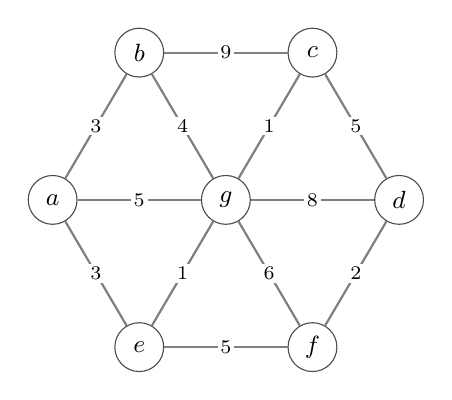
\begin{tikzpicture}[x=1.1cm, y=1.1cm]
\node[mst-v] (v1) at (-2,0) {$a$};
\node[mst-v] (v2) at (-1,1.7) {$b$};
\node[mst-v] (v3) at (1,1.7) {$c$};
\node[mst-v] (v4) at (2,0) {$d$};
\node[mst-v] (v6) at (1,-1.7) {$f$};
\node[mst-v] (v5) at (-1,-1.7) {$e$};
\node[mst-v] (v7) at (0,0) {$g$};
\draw[mst-e] (v1) -- node[mst-w] {3} (v2);
\draw[mst-e] (v2) -- node[mst-w] {9} (v3);
\draw[mst-e] (v3) -- node[mst-w] {5} (v4);
\draw[mst-e] (v4) -- node[mst-w] {2} (v6);
\draw[mst-e] (v5) -- node[mst-w] {5} (v6);
\draw[mst-e] (v1) -- node[mst-w] {3} (v5);
\draw[mst-e] (v1) -- node[mst-w] {5} (v7);
\draw[mst-e] (v2) -- node[mst-w] {4} (v7);
\draw[mst-e] (v3) -- node[mst-w] {1} (v7);
\draw[mst-e] (v4) -- node[mst-w] {8} (v7);
\draw[mst-e] (v5) -- node[mst-w] {1} (v7);
\draw[mst-e] (v6) -- node[mst-w] {6} (v7);
\end{tikzpicture}
\diagcaption{觀念題用的圖 $H$。}
\label{fig:mst-h}
\end{minipage}
\end{center}

\begin{enumerate}
\item \label{q:mst-choice}（選擇，可能不只一個答案）$G$ 是連通的加權無向圖，至少有三條邊。 下
列哪些敘述正確？
\begin{enumerate}
\item 權重互不相同時，權重第二小的邊一定在最小生成樹裡。
\item 權重互不相同時，權重第三小的邊一定在最小生成樹裡。
\item 每個頂點連出去的邊裡最重的那一條，一定不在任何最小生成樹裡。
\item 每條邊的權重都加上同一個常數 $c$（$c$ 可以是負數），最小生成樹的邊集合不變。
\item 權重有正有負時，把每個權重換成它的平方，最小生成樹的邊集合不變。
\item Prim 演算法在有負權重的圖上仍然正確。
\item 最小生成樹上任兩點之間的路徑，就是兩點之間的最短路徑。
\item 最小生成樹只有一棵，則權重一定互不相同。
\item Sollin 演算法某一回合開始時有 $k \ge 2$ 個元件，這一回合至少加入 $\lceil k/2 \rceil$ 條邊。
\end{enumerate}

\item \label{q:mst-kruskal-h}（追蹤）對 $H$ 執行 Kruskal 演算法。 依序寫出看過的每一條邊、選或
略過（略過的寫原因），以及最小生成樹的總權重。

\item \label{q:mst-prim-h}（追蹤）對 $H$ 從 $a$ 開始執行 Prim 演算法。 (a) 照本章的格式寫出每一
回合的 $\mathit{key}/\pi$ 表和加入的邊。 (b) 有哪幾個回合遇到 $\mathit{key}$ 平手？ 平手規則
決定了什麼？ (c) \proc{Decrease-Key} 一共做了幾次？

\item \label{q:mst-lazy-h}（計算）對 $H$ 從 $a$ 開始執行虛擬碼~\ref{alg:mst-prim-lazy}（三元組先
比權重、再比頂點字母）。 \proc{Insert} 一共做了幾次？ 取出的資料有幾筆是過期的？ 堆積裡最
多同時有幾筆？ 和上一題的 \proc{Decrease-Key} 次數比較。

\item \label{q:mst-sollin-h}（追蹤）對 $H$ 執行 Sollin 演算法。 (a) 寫出每一回合每個元件挑的邊和
這一回合加入的邊。 (b) 第一回合頂點 $g$ 的兩條權重 $1$ 的邊平手。 如果 $g$ 改挑另一條，這一
回合加入的邊會不會不同？

\item \label{q:mst-count-h}（計算）(a) $H$ 有幾棵最小生成樹？ 全部列出。 (b) Kruskal 演算法在權
重相同時改成「照 $\prec$ 倒過來的順序」，會得到哪一棵？

\item \label{q:mst-second-h}（計算）令 $T$ 是第~\ref{q:mst-kruskal-h}~題的最小生成樹。 (a) 對每
一條非樹邊，寫出它和 $T$ 形成的環上最重的樹邊，以及換進來之後的總權重。 (b) 依「和 $T$ 不同
的生成樹裡最輕的」的定義，次小生成樹的總權重是多少？ (c) 依「總權重嚴格大於最小生成樹」的定
義呢？

\item \label{q:mst-spt-h}（計算）(a) 寫出 $H$ 裡從 $a$ 到每個頂點的最短距離 $\delta(a, v)$。 (b)
以 $a$ 為根的最短路徑樹有幾棵？ 它們的總權重各是多少？ (c) 其中有沒有哪一棵也是最小生成樹？
(d) 在第~\ref{q:mst-kruskal-h}~題的最小生成樹上，$a$ 到 $f$ 的路徑長是多少？ 和 $\delta(a, f)$
比較。

\item \label{q:mst-two-light}（證明）$G$ 是權重互不相同的連通圖，$n \ge 3$。 (a) 證明權重最小和
第二小的兩條邊都在最小生成樹裡。 (b) 舉一個例子，權重第三小的邊不在最小生成樹裡。 (c) 對每個頂
點，取它連出去的邊裡最輕的一條。 證明這些邊都在最小生成樹裡，而且其中不同的邊至少有 $\lceil
n/2 \rceil$ 條。

\item \label{q:mst-unique-iff}（證明）證明系理~\ref{cor:mst-unique-iff}：最小生成樹 $T$ 是唯一
的，若且唯若每一條非樹邊 $(x, y)$ 都滿足 $w(x, y) > \mathit{max}_T(x, y)$。（提示：$\Leftarrow$
可以模仿定理~\ref{thm:mst-check} 的證明，或用環性質。）

\item \label{q:mst-max}（證明）(a) Kruskal 演算法改成依權重由大到小排序，其他不變。 證明它得
到總權重最大的生成樹。 (b) 一條路徑上最輕的邊叫它的「寬度」（例如管線的最小管徑）。 證明：
在總權重最大的生成樹上，任兩點之間的路徑，是兩點之間所有路徑裡寬度最大的。

\item \label{q:mst-dense}（選擇與計算）下面三種情況，各用本章哪一種寫法最合適？ 估計大約要幾
步。 (a) $n = 3000$ 的完全圖。 (b) $n = 2 \times 10^5$、$m = 4 \times 10^5$ 的道路網。 (c) $n =
10^6$、$m = 3 \times 10^6$，邊已經依權重由小到大排好。

\item \label{q:mst-rounds}（計算）(a) $n$ 個頂點排成一條路徑 $1, 2, \ldots, n$，邊 $(i, i + 1)$
的權重是 $i$。 Sollin 演算法要幾回合？ (b) 畫一張 $8$ 個頂點的連通圖，讓 Sollin 演算法恰好要
$3$ 回合（定理~\ref{thm:mst-rounds} 的上限），並寫出每回合加入的邊。
\end{enumerate}

\section{實作練習}
\label{sec:mst-practice}

下面是 Aki-Judge 上和本章相關的題目。 Sollin 演算法目前沒有題目，可以把
範例~\ref{ex:mst-sollin} 的輸出拿掉，改成只印總權重，拿前兩題的測資驗證。

\begin{center}
\begin{tabular}{llc}
\toprule
小節 & 題目 & 難度 \\
\midrule
Kruskal & \akiref{total-weight-of-a-minimum-spanning-tree}{最小生成樹的總權重} & 基本 \\
Kruskal & \akiref{mst-total-weight-on-a-connected-graph}{連通圖的最小生成樹總權重} & 基本 \\
Kruskal & \akiref{compare-two-kruskal-runs}{兩次 Kruskal 的總權重比較} & 基本 \\
Prim & \akiref{minimum-spanning-tree-grown-from-vertex-1}{從頂點 1 擴張的最小生成樹} & 基本 \\
瓶頸 & \akiref{smallest-threshold-connecting-first-and-last-vertex}{使頂點 1 與 n 連通的最小門檻} & 進階 \\
\bottomrule
\end{tabular}
\end{center}

幾題的提示：

\begin{itemize}
\item 「最小生成樹的總權重」和「連通圖的最小生成樹總權重」都是範例~\ref{ex:mst-kruskal} 拿掉
逐邊輸出；前一題的 $n$、$m$ 比較大，排序和互斥集合都要用本章的寫法。 總和用 \texttt{long
long}。
\item 「兩次 Kruskal 的總權重比較」要把 Kruskal 寫成一個函式，每次呼叫前重新初始化互斥集合。
用同一份邊陣列呼叫兩次時，第二次拿到的是已經排好的陣列，結果一樣。
\item 「從頂點 1 擴張的最小生成樹」的 $n$ 最多 $2000$，範例~\ref{ex:mst-prim-heap} 和
範例~\ref{ex:mst-prim-array} 都夠快；每回合重新掃過所有的邊找最輕的寫法是 $O(nm)$，才會太
慢。 輸入有自環，兩個範例都已經處理。
\item 「使頂點 1 與 n 連通的最小門檻」問的是瓶頸，不是最短路徑。 照
定理~\ref{thm:mst-bottleneck} 後面的說明，Kruskal 由輕到重加邊，$1$ 和 $n$ 第一次連通時加進來
的那條邊的權重就是答案；$n = 1$ 時答案是 $0$。
\end{itemize}

\section{讀完你應該會}
\label{sec:mst-checklist}

\begin{itemize}
\item 說出切割、輕邊、安全的邊的定義，用換邊論證證明切割性質和環性質。
\item 手算 Kruskal 演算法的選邊表（跳過的邊寫出原因），以及 Prim 演算法的 $\mathit{key}/\pi$
表，說明兩者選邊的順序為什麼不同。
\item 比較 Prim 演算法三種寫法（帶索引堆積、允許重複放入、陣列）的時間和空間，判斷稠密圖、
稀疏圖各該用哪一種。
\item 手算 Sollin 演算法每回合每個元件挑的邊，說明平手規則為什麼要一致，以及回合數為什麼不
超過 $\lfloor \lg n \rfloor$。
\item 證明權重互不相同時最小生成樹唯一，用非樹邊的條件判斷一棵生成樹是不是（唯一的）最小生
成樹，用換邊求次小生成樹。
\item 舉反例說明最小生成樹不是最短路徑樹，知道最小生成樹上的路徑是瓶頸最小的路徑。
\end{itemize}

\textbf{延伸閱讀}（書末會整理完整的參考資料）

\begin{itemize}
\item Thomas H. Cormen 等，\textit{Introduction to Algorithms}，第 4 版，第 21 章：用安全的邊
統一說明 Kruskal 和 Prim，章末的問題討論次小生成樹、瓶頸生成樹和稀疏圖的加速。
\item Joseph B. Kruskal，``On the Shortest Spanning Subtree of a Graph and the Traveling
Salesman Problem''，\textit{Proceedings of the American Mathematical Society} 7(1)，1956：
Kruskal 演算法的原始論文，只有三頁。
\item Robert C. Prim，``Shortest Connection Networks and Some Generalizations''，\textit{Bell
System Technical Journal} 36(6)，1957。 同一個方法更早由 Vojtěch Jarník 在 1930 年發表，所以
也叫 Jarník 演算法。
\item Otakar Borůvka，``O jistém problému minimálním''，\textit{Práce moravské
přírodovědecké společnosti} 3，1926：Sollin 演算法的最早版本（捷克文）。
\item R. L. Graham、Pavol Hell，``On the History of the Minimum Spanning Tree Problem''，
\textit{Annals of the History of Computing} 7(1)，1985：三個演算法誰先誰後的完整考證。
\item Robert E. Tarjan，\textit{Data Structures and Network Algorithms}，SIAM，1983，第 6 章：
用「藍色規則」（切割性質）和「紅色規則」（環性質）統一所有最小生成樹演算法。
\item David R. Karger、Philip N. Klein、Robert E. Tarjan，``A Randomized Linear-Time
Algorithm to Find Minimum Spanning Trees''，\textit{Journal of the ACM} 42(2)，1995：期望時間
$O(m)$ 的演算法，用到 Sollin 的回合和第~\ref{sec:mst-more}~節的判定定理。
\item Steven S. Skiena，\textit{The Algorithm Design Manual}，第 3 版，8.1 節：最小生成樹的
應用和變形，偏重怎麼把實際問題換成最小生成樹。
\end{itemize}

\addcontentsline{toc}{section}{觀念題解答}
\section*{觀念題解答}

\begin{enumerate}
\item (a)、(d)、(f)、(i) 正確。 (a)：最輕的兩條邊不會形成環（環至少三條邊），Kruskal 演算法
一定選它們；權重互不相同時最小生成樹唯一，所以它們在最小生成樹裡。 (b)：三角形的三條邊權重
$1, 2, 3$，第三小的是環上最重的，不選。 (c)：一個度數 $1$ 的頂點只有一條邊，它既是最重也是最
輕，一定要選。 (d)：每棵生成樹都恰好 $n - 1$ 條邊，總權重都加 $(n - 1)c$，大小順序不變。 (e)：
三角形權重 $-3, 1, 2$，原本選 $-3, 1$；平方後是 $9, 1, 4$，改選 $1, 4$，也就是原本的 $1, 2$。
(f)：定理~\ref{thm:mst-prim} 的證明沒有用到權重的正負。 (g)：圖~\ref{fig:mst-spt}。 (h)：
第~\ref{sec:mst-props}~節權重 $1, 1, 2$ 的三角形。 (i)：$k$ 個元件各挑一條邊，每條邊最多被兩
個元件挑到，所以不同的邊至少 $\lceil k/2 \rceil$ 條；由定理~\ref{thm:mst-sollin}，它們都會被
加入。

\item 照 $\prec$ 排序：$c$--$g$（$1$）、$e$--$g$（$1$）、$d$--$f$（$2$）、$a$--$b$（$3$）、
$a$--$e$（$3$）、$b$--$g$（$4$）、$a$--$g$（$5$）、$c$--$d$（$5$）、$e$--$f$（$5$）、
$f$--$g$（$6$）、$d$--$g$（$8$）、$b$--$c$（$9$）。

\begin{center}
\small
\begin{tabular}{rcrl}
\toprule
步 & 邊 & 權重 & 結果 \\
\midrule
1 & $c$--$g$ & 1 & 選 \\
2 & $e$--$g$ & 1 & 選 \\
3 & $d$--$f$ & 2 & 選 \\
4 & $a$--$b$ & 3 & 選 \\
5 & $a$--$e$ & 3 & 選（$\{a, b\}$ 和 $\{c, e, g\}$ 合併） \\
6 & $b$--$g$ & 4 & 略過：$b$、$g$ 已經經過 $a, e$ 連通 \\
7 & $a$--$g$ & 5 & 略過：$a$、$g$ 已經經過 $e$ 連通 \\
8 & $c$--$d$ & 5 & 選，已滿 $6$ 條 \\
\bottomrule
\end{tabular}
\end{center}
後面四條不用看。 最小生成樹是 $\{c\text{--}g, e\text{--}g, d\text{--}f, a\text{--}b, a\text{--}e,
c\text{--}d\}$，總權重 $1 + 1 + 2 + 3 + 3 + 5 = 15$。

\item (a)
\begin{center}
\footnotesize
\setlength{\tabcolsep}{3.2pt}
\setlength{\fboxsep}{1.2pt}
\begin{tabular}{cccrrrrrrr}
\toprule
回合 & 取出 & 加入的邊 & $a$ & $b$ & $c$ & $d$ & $e$ & $f$ & $g$ \\
\midrule
1 & $a$ & — & \mstsel{$0$} & \mstchg{$3/a$} & $\infty$ & $\infty$ & \mstchg{$3/a$} & $\infty$ & \mstchg{$5/a$} \\
2 & $b$ & $a$--$b$ &  & \mstsel{$3/a$} & \mstchg{$9/b$} & $\infty$ & $3/a$ & $\infty$ & \mstchg{$4/b$} \\
3 & $e$ & $a$--$e$ &  &  & $9/b$ & $\infty$ & \mstsel{$3/a$} & \mstchg{$5/e$} & \mstchg{$1/e$} \\
4 & $g$ & $e$--$g$ &  &  & \mstchg{$1/g$} & \mstchg{$8/g$} &  & $5/e$ & \mstsel{$1/e$} \\
5 & $c$ & $g$--$c$ &  &  & \mstsel{$1/g$} & \mstchg{$5/c$} &  & $5/e$ &  \\
6 & $d$ & $c$--$d$ &  &  &  & \mstsel{$5/c$} &  & \mstchg{$2/d$} &  \\
7 & $f$ & $d$--$f$ &  &  &  &  &  & \mstsel{$2/d$} &  \\
\bottomrule
\end{tabular}
\end{center}
加入的邊依序是 $a$--$b$、$a$--$e$、$e$--$g$、$g$--$c$、$c$--$d$、$d$--$f$，總權重 $15$，和上一題
同一棵樹。 (b) 第 2 回合 $b$、$e$ 的 $\mathit{key}$ 都是 $3$，取字母小的 $b$；這只影響順序，兩
條邊最後都會選。 第 6 回合 $d$、$f$ 的 $\mathit{key}$ 都是 $5$，取 $d$，於是加入 $c$--$d$，之後
$f$ 改經由 $d$--$f$（$2$）接進來；如果先取 $f$，加入的是 $e$--$f$，$d$ 再經由 $d$--$f$ 接進
來，得到另一棵最小生成樹（第~\ref{q:mst-count-h}~題）。 (c) 表裡有底色的格子共 $11$ 個，也就
是 $11$ 次；其中第一次把 $\infty$ 改小的有 $6$ 次，真正把有限的值再改小的有 $5$ 次（$g$ 兩次，
$c$、$d$、$f$ 各一次）。

\item \proc{Insert} 共 $13$ 次（$12$ 條邊各一次，加上起點）。 取出的順序是 $(0, a)$、$(3, b)$、
$(3, e)$、$(1, g)$、$(1, c)$、$(4, g)$ 過期、$(5, d)$、$(2, f)$，之後 $(5, f)$、$(5, g)$、$(6, f)$、
$(8, d)$、$(9, c)$ 都過期，共 $6$ 筆過期（加入第 $7$ 個頂點後就可以停，不用取出最後五筆）。 堆
積最多同時有 $7$ 筆，發生在取出 $g$、放入 $(1, c)$、$(8, d)$、$(6, f)$ 之後。 帶索引的版本做
了 $11$ 次 \proc{Decrease-Key}，堆積最多 $7$ 個頂點；這裡多做了兩次插入，堆積大小差不多。 圖
大的時候差別在空間：一個是 $\Theta(m)$，一個是 $\Theta(n)$。

\item (a) 第一回合：
\begin{center}
\small
\begin{tabular}{ccccccc}
\toprule
$\{a\}$ & $\{b\}$ & $\{c\}$ & $\{d\}$ & $\{e\}$ & $\{f\}$ & $\{g\}$ \\
\midrule
$a$--$b$（$3$） & $a$--$b$（$3$） & $c$--$g$（$1$） & $d$--$f$（$2$） & $e$--$g$（$1$） & $d$--$f$（$2$） &
$c$--$g$（$1$） \\
\bottomrule
\end{tabular}
\end{center}
$a$ 的 $a$--$b$、$a$--$e$ 平手，$(3, a, b) \prec (3, a, e)$；$g$ 的 $c$--$g$、$e$--$g$ 平手，取
$c$--$g$。 加入 $a$--$b$、$c$--$g$、$d$--$f$、$e$--$g$，剩三個元件 $\{a, b\}$、$\{c, e, g\}$、
$\{d, f\}$。 第二回合：$\{a, b\}$ 挑 $a$--$e$（$3$）；$\{c, e, g\}$ 也挑 $a$--$e$（$3$）；
$\{d, f\}$ 的 $c$--$d$、$e$--$f$ 都是 $5$，$(5, c, d) \prec (5, e, f)$，挑 $c$--$d$。 加入
$a$--$e$、$c$--$d$，結束，總權重 $15$，和第~\ref{q:mst-kruskal-h}~題同一棵（定理~\ref{thm:mst-sollin}）。
(b) 不會。 $c$ 自己挑 $c$--$g$、$e$ 自己挑 $e$--$g$，兩條本來就都會加入，$g$ 挑哪一條都只是重
複。

\item (a) 兩棵。 $c$--$g$、$e$--$g$、$d$--$f$、$a$--$b$、$a$--$e$ 是兩棵共同的：前三條是各自
頂點唯一最輕的邊；$a$--$b$ 是 $b$ 和其他頂點之間的切割裡唯一最輕的（$b$ 的邊是 $3, 4, 9$）；
$a$--$e$ 是切割 $(\{a, b\}, \{c, \ldots, g\})$ 唯一最輕的（跨越的邊是 $3, 4, 5, 9$）。 剩下要把
$\{d, f\}$ 接上 $\{a, b, c, e, g\}$，跨越的邊是 $c$--$d$（$5$）、$e$--$f$（$5$）、$f$--$g$（$6$）、
$d$--$g$（$8$），選 $c$--$d$ 或 $e$--$f$ 都是總權重 $15$。 兩棵分別是第~\ref{q:mst-kruskal-h}~題
的樹，以及把其中的 $c$--$d$ 換成 $e$--$f$。 (b) 權重 $5$ 的三條邊順序倒過來，變成 $e$--$f$、
$c$--$d$、$a$--$g$，先看到 $e$--$f$ 就選它，得到第二棵。

\item (a)
\begin{center}
\small
\begin{tabular}{clcc}
\toprule
非樹邊 & $T$ 上的路徑 & 環上最重的樹邊 & 換進來的總權重 \\
\midrule
$b$--$g$（$4$） & $b, a, e, g$ & $a$--$b$ 或 $a$--$e$（$3$） & $16$ \\
$a$--$g$（$5$） & $a, e, g$ & $a$--$e$（$3$） & $17$ \\
$e$--$f$（$5$） & $e, g, c, d, f$ & $c$--$d$（$5$） & $15$ \\
$f$--$g$（$6$） & $f, d, c, g$ & $c$--$d$（$5$） & $16$ \\
$d$--$g$（$8$） & $d, c, g$ & $c$--$d$（$5$） & $18$ \\
$b$--$c$（$9$） & $b, a, e, g, c$ & $a$--$b$ 或 $a$--$e$（$3$） & $21$ \\
\bottomrule
\end{tabular}
\end{center}
(b) $15$：換進 $e$--$f$、拿掉 $c$--$d$，得到另一棵最小生成樹。 (c) $16$。 $e$--$f$ 和環上最重的
$c$--$d$ 一樣重，照作答提醒改拿環上嚴格比 $5$ 輕的最重的邊 $d$--$f$（$2$），得 $15 + 5 - 2 =
18$；其他各列不變。 最小的是 $16$，從 $T$ 換一條邊得到的有三棵：換進 $b$--$g$ 拿掉 $a$--$b$ 或 $a$--$e$，或換進
$f$--$g$ 拿掉 $c$--$d$。

\item (a) $\delta(a, b) = 3$、$\delta(a, e) = 3$、$\delta(a, g) = 4$（$a, e, g$）、$\delta(a, c) =
5$（$a, e, g, c$）、$\delta(a, f) = 8$（$a, e, f$）、$\delta(a, d) = 10$。 (b) 兩棵。 $b, e, g, c,
f$ 的最短路徑都只有一條；$d$ 可以經過 $c$（$5 + 5$）或經過 $f$（$8 + 2$）。 共同的邊是
$a$--$b$、$a$--$e$、$e$--$g$、$g$--$c$、$e$--$f$，總權重 $13$，再加 $c$--$d$ 是 $18$，加
$d$--$f$ 是 $15$。 (c) 有。 加 $d$--$f$ 的那一棵總權重 $15$，正是第~\ref{q:mst-count-h}~題的第
二棵最小生成樹。 這是巧合，不是規則：圖~\ref{fig:mst-spt} 的最短路徑樹就比最小生成樹重。 (d)
第~\ref{q:mst-kruskal-h}~題的樹上 $a$ 到 $f$ 走 $a, e, g, c, d, f$，長 $3 + 1 + 1 + 5 + 2 = 12$，
比 $\delta(a, f) = 8$ 長。

\item (a) 最輕的邊 $e_1$ 自己不會形成環，Kruskal 演算法第一個選它。 第二輕的 $e_2$ 和 $e_1$ 最多
共用一個端點，兩條邊不會形成環（簡單圖的環至少三條邊），所以第二個也選。 權重互不相同，最小
生成樹唯一（定理~\ref{thm:mst-unique}），就是 Kruskal 選的那一棵。 (b) 三角形，權重 $1, 2, 3$；
或任何一個三條最輕的邊剛好圍成三角形的圖。 (c) 頂點 $v$ 最輕的邊是切割 $(\{v\}, V - \{v\})$ 唯
一的輕邊，由系理~\ref{cor:mst-cut-strict}，它在最小生成樹裡。 $n$ 個頂點各取一條，一條邊最多
被它的兩個端點取到，所以不同的邊至少 $\lceil n/2 \rceil$ 條。

\item $\Rightarrow$：假設某條非樹邊 $(x, y)$ 有 $w(x, y) \le \mathit{max}_T(x, y)$。 由
定理~\ref{thm:mst-check}，$T$ 是最小生成樹，所以 $w(x, y) \ge \mathit{max}_T(x, y)$，兩者相等。
令 $f$ 是 $P_T(x, y)$ 上權重等於 $w(x, y)$ 的樹邊，$T - \{f\} \cup \{(x, y)\}$ 是另一棵生成樹，
總權重相同，也是最小生成樹，和唯一矛盾。

$\Leftarrow$：設每條非樹邊都嚴格比 $\mathit{max}_T$ 重，而 $T' \ne T$ 也是最小生成樹。 取一
條 $f = (x, y) \in T' - T$。 從 $T'$ 拿掉 $f$ 分成兩塊，$P_T(x, y)$ 有一條樹邊 $e$ 跨越這兩塊，
$e \notin T'$。 由假設 $w(f) > \mathit{max}_T(x, y) \ge w(e)$，$T' - \{f\} \cup \{e\}$ 比 $T'$ 輕，
矛盾。 所以 $T$ 是唯一的最小生成樹。

\item (a) 令 $w''(e) = -w(e)$。 由重到輕排 $w$ 就是由輕到重排 $w''$，演算法的每一步都和「在
$w''$ 上執行原本的 Kruskal」相同，所以得到 $w''$ 的最小生成樹 $T$。 對任何生成樹 $T_1$，
$w''(T) \le w''(T_1)$，也就是 $w(T) \ge w(T_1)$。 本章的證明沒有用到權重的正負，所以換成負的
權重也成立。 (b) 由 (a)，總權重最大的生成樹 $T$ 是 $w''$ 的最小生成樹。 對 $w''$ 用
定理~\ref{thm:mst-bottleneck}：任何 $x$ 到 $y$ 的路徑 $Q$ 上 $w''$ 最大的邊，至少是 $T$ 的路徑上
$w''$ 最大的邊。 $w''$ 最大就是 $w$ 最小，所以 $Q$ 上 $w$ 最小的邊，至多是 $T$ 的路徑上 $w$ 最小
的邊，也就是 $Q$ 的寬度不超過 $T$ 上路徑的寬度。

\item (a) 完全圖 $m = n(n - 1)/2 \approx 4.5 \times 10^6$，是稠密圖，用陣列版 Prim，大約 $2n^2 =
1.8 \times 10^7$ 步，不用存邊。 堆積版最壞大約 $m \lg n \approx 5 \times 10^7$；Kruskal 光排序
就要 $m \lg m \approx 10^8$ 次比較，還要先存下 $4.5 \times 10^6$ 條邊。 (b) 稀疏圖，用堆積版
Prim 或 Kruskal：前者大約 $(n + m) \lg n \approx 6 \times 10^5 \times 18 \approx 10^7$，後者排
序大約 $m \lg m \approx 7.4 \times 10^6$；陣列版要 $n^2 = 4 \times 10^{10}$ 步，不能用。 (c) 用
Kruskal，邊已經排好就省掉排序，只剩 $m$ 次左右的互斥集合操作，$O(m\,\alpha(n))$，大約幾百萬
步；Prim 至少要 $(n + m) \lg n \approx 8 \times 10^7$。

\item (a) $1$ 回合。 頂點 $1$ 只有邊 $(1, 2)$；頂點 $i \ge 2$ 的兩條邊權重是 $i - 1$ 和 $i$，挑
$(i - 1, i)$。 所以每條邊都被挑到，第一回合就加入全部 $n - 1$ 條邊。 這說明定理~\ref{thm:mst-rounds}
只是上限，回合數可以遠少於 $\lg n$。 (b) 一個例子：路徑 $1, 2, \ldots, 8$，七條邊依序的權重是
$1, 10, 2, 20, 3, 11, 4$（$(1, 2)$ 是 $1$、$(2, 3)$ 是 $10$、$(3, 4)$ 是 $2$，依此類推）。 第一回合每
個頂點挑它在 $\{1, 2\}$、$\{3, 4\}$、$\{5, 6\}$、$\{7, 8\}$ 裡那條邊，加入 $1$--$2$、$3$--$4$、
$5$--$6$、$7$--$8$。 第二回合 $\{1, 2\}$ 和 $\{3, 4\}$ 都挑 $2$--$3$（$10$，比 $4$--$5$ 的 $20$
輕），$\{5, 6\}$ 和 $\{7, 8\}$ 都挑 $6$--$7$（$11$），加入兩條，剩 $\{1, 2, 3, 4\}$、$\{5, 6, 7,
8\}$。 第三回合兩邊都挑 $4$--$5$。 共 $3$ 回合。
\end{enumerate}
